% =====================================================================
%  PAPER II -- SoK: The Quantifier Gap Between Certified Robustness
%              and Airworthiness Assurance
%
%  Target venue : IEEE Symposium on Security and Privacy, SoK track
%  Class        : IEEEtran (conference). Overleaf ships IEEEtran.
%  Build        : latexmk -pdf main.tex      (pdfLaTeX + BibTeX)
%
%  Every number quoted in the text is a macro from numbers.tex, generated
%  by paperII/experiments/make_numbers.py from committed result CSVs.
%  The transfer, objective and reliability table bodies are generated too.
%  Do not edit numbers by hand: re-run paperII/experiments/run_all.sh.
% =====================================================================
\documentclass[conference,letterpaper,10pt]{IEEEtran}
\IEEEoverridecommandlockouts
\usepackage{mathptmx}
\usepackage{cite}
\usepackage{amsmath,amssymb,amsfonts}
\usepackage{amsthm}
\usepackage{graphicx}
\usepackage{booktabs}
\usepackage{tabularx}
\usepackage{array}
\usepackage{multirow}
\usepackage[table]{xcolor}
\usepackage{tikz}
\usepackage{pgfplots}
\pgfplotsset{compat=1.17}
\usepgfplotslibrary{groupplots}
\usetikzlibrary{arrows.meta,positioning,fit,backgrounds,shapes.geometric,calc}
\usepackage{enumitem}
\usepackage[hidelinks]{hyperref}

% Generated by paperII/experiments/make_numbers.py -- do not edit by hand.
\newcommand{\nCorpus}{86}
\newcommand{\nTierA}{46}
\newcommand{\nTierB}{40}
\newcommand{\nObj}{22}
\newcommand{\nObjPrimary}{14}
\newcommand{\nClasses}{17}
\newcommand{\hOnePercInAB}{64\,\%}
\newcommand{\hOnePercInA}{14\,\%}
\newcommand{\hOneCtrlTrAB}{56\,\%}
\newcommand{\hOneCtrlTrA}{57\,\%}
\newcommand{\hOneCtrlInAB}{19\,\%}
\newcommand{\hOneAllInAB}{41\,\%}
\newcommand{\hOneNPercAB}{44}
\newcommand{\hOneNCtrlAB}{32}
\newcommand{\hOneNPercA}{14}
\newcommand{\hOneNCtrlA}{23}
\newcommand{\hOnePercInCount}{28}
\newcommand{\hTwoNLifted}{54}
\newcommand{\hTwoShareU}{4\,\%}
\newcommand{\hTwoShareS}{80\,\%}
\newcommand{\hTwoShareSe}{4\,\%}
\newcommand{\hTwoShareSec}{13\,\%}
\newcommand{\hTwoAccounted}{17\,\%}
\newcommand{\hTwoConf}{13\,\%}
\newcommand{\hTwoAccEarly}{7\,\%}
\newcommand{\hTwoAccLate}{26\,\%}
\newcommand{\hTwoNEarly}{27}
\newcommand{\hTwoNLate}{27}
\newcommand{\hTwoDynN}{25}
\newcommand{\hTwoDynAcc}{16\,\%}
\newcommand{\hTwoGenN}{11}
\newcommand{\hTwoGenAcc}{45\,\%}
\newcommand{\hTwoConcN}{20}
\newcommand{\hTwoConcAcc}{35\,\%}
\newcommand{\hTwoMonN}{9}
\newcommand{\hTwoMonAcc}{0\,\%}
\newcommand{\hTwoSupN}{0}
\newcommand{\hTwoRateN}{3}
\newcommand{\hThreeNP}{20}
\newcommand{\hThreePercP}{12}
\newcommand{\hThreePercShareP}{27\,\%}
\newcommand{\hThreeCtrlP}{1}
\newcommand{\hThreeEstShareP}{83\,\%}
\newcommand{\hThreeNRate}{3}
\newcommand{\hThreePercPA}{5}
\newcommand{\ttCells}{102}
\newcommand{\ttD}{8}
\newcommand{\ttL}{66}
\newcommand{\ttX}{28}
\newcommand{\ttTOneReach}{15}
\newcommand{\ttTOneMinK}{1}
\newcommand{\ttTFourD}{1}
\newcommand{\ttTSixD}{0}
\newcommand{\hFourReach}{11}
\newcommand{\hFourRtaDeficit}{4}
\newcommand{\relScopeAgree}{88\,\%}
\newcommand{\relScopeKappa}{0.83}
\newcommand{\relScopeAlpha}{0.83}
\newcommand{\relScopeAcOne}{0.85}
\newcommand{\relScopePabak}{0.84}
\newcommand{\relScopeAlphaLo}{0.72}
\newcommand{\relScopeAlphaHi}{0.92}
\newcommand{\relModAgree}{93\,\%}
\newcommand{\relModKappa}{0.88}
\newcommand{\relModAlpha}{0.88}
\newcommand{\relModAcOne}{0.92}
\newcommand{\relModPabak}{0.91}
\newcommand{\relModAlphaLo}{0.78}
\newcommand{\relModAlphaHi}{0.96}
\newcommand{\relTypeAgree}{86\,\%}
\newcommand{\relTypeKappa}{0.83}
\newcommand{\relTypeAlpha}{0.83}
\newcommand{\relTypeAcOne}{0.85}
\newcommand{\relTypePabak}{0.85}
\newcommand{\relTypeAlphaLo}{0.74}
\newcommand{\relTypeAlphaHi}{0.91}
\newcommand{\relAssmAgree}{85\,\%}
\newcommand{\relAssmKappa}{0.47}
\newcommand{\relAssmAlpha}{0.46}
\newcommand{\relAssmAcOne}{0.83}
\newcommand{\relAssmPabak}{0.80}
\newcommand{\relAssmAlphaLo}{0.21}
\newcommand{\relAssmAlphaHi}{0.67}
\newcommand{\relPertAgree}{76\,\%}
\newcommand{\relPertKappa}{0.70}
\newcommand{\relPertAlpha}{0.69}
\newcommand{\relPertAcOne}{0.72}
\newcommand{\relPertPabak}{0.72}
\newcommand{\relPertAlphaLo}{0.57}
\newcommand{\relPertAlphaHi}{0.80}
\newcommand{\relTierAgree}{92\,\%}
\newcommand{\relTierKappa}{0.84}
\newcommand{\relTierAlpha}{0.84}
\newcommand{\relTierAcOne}{0.84}
\newcommand{\relTierPabak}{0.84}
\newcommand{\relTierAlphaLo}{0.70}
\newcommand{\relTierAlphaHi}{0.93}
\newcommand{\relCompAgree}{90\,\%}
\newcommand{\relCompKappa}{0.82}
\newcommand{\relCompAlpha}{0.82}
\newcommand{\relCompAcOne}{0.88}
\newcommand{\relCompPabak}{0.87}
\newcommand{\relCompAlphaLo}{0.71}
\newcommand{\relCompAlphaHi}{0.92}
\newcommand{\relEvidAgree}{88\,\%}
\newcommand{\relEvidKappa}{0.77}
\newcommand{\relEvidAlpha}{0.77}
\newcommand{\relEvidAcOne}{0.86}
\newcommand{\relEvidPabak}{0.84}
\newcommand{\relEvidAlphaLo}{0.62}
\newcommand{\relEvidAlphaHi}{0.89}
\newcommand{\relJaccard}{0.90}
\newcommand{\relNDisagree}{88}
\newcommand{\relNDisPapers}{53}
\newcommand{\adjN}{50}
\newcommand{\adjPapers}{37}
\newcommand{\rateDecisionsPerH}{108{,}000}
\newcommand{\ratePstarThirty}{9.3\times10^{-10}}
\newcommand{\ratePstarKThree}{9.7\times10^{-4}}
\newcommand{\ratePstarNine}{9.3\times10^{-15}}
\newcommand{\rateGainIndep}{1\times10^{6}}
\newcommand{\rateGainMin}{6.75}
\newcommand{\rateGainMax}{111}
\newcommand{\rateGainBound}{6.75}
\newcommand{\ecoHoursFour}{29{,}957}
\newcommand{\ecoFramesFour}{3.2\times10^{9}}
\newcommand{\ecoYearsSeven}{3{,}417}
\newcommand{\ecoYearsNine}{3.4\times10^{5}}
\newcommand{\epTubeEkf}{2.22}
\newcommand{\epTubeSup}{2.65}
\newcommand{\epTubeKin}{24.4}
\newcommand{\epDeltaPos}{0.68}
\newcommand{\epGammaEkf}{1.365}
\newcommand{\epGammaSup}{1.625}
\newcommand{\epNObl}{6}
\newcommand{\epNOpen}{2}


% ---------------- notation -------------------------------------------
\newcommand{\prov}[1]{\textsc{\footnotesize #1}}
% expandable input for generated table bodies (avoids "Misplaced \noalign")
\makeatletter\newcommand{\inputbody}[1]{\@@input #1 }\makeatother
% quantifier types: \Q{scope}{modality}
\newcommand{\scin}{\mathsf{in}}
\newcommand{\sctr}{\mathsf{tr}}
\newcommand{\scop}{\mathsf{op}}
\newcommand{\scpopd}{\mathsf{pop}_{\mathsf{d}}}
\newcommand{\scpoph}{\mathsf{pop}_{\mathsf{h}}}
\newcommand{\scpop}{\mathsf{pop}}
\newcommand{\modA}{\forall}
\newcommand{\modAc}{\forall_{\!\alpha}}
\newcommand{\modP}{\mathbb{P}}
\newcommand{\modE}{\mathbb{E}}
\newcommand{\modX}{\exists}
\newcommand{\Q}[2]{\ensuremath{\langle\csname sc#1\endcsname,\csname mod#2\endcsname\rangle}}
\newcommand{\lift}[1]{\ensuremath{\mathsf{L}_{\mathrm{#1}}}}
\newcommand{\obl}[1]{\ensuremath{\mathsf{O}_{\mathrm{#1}}}}
\newcommand{\Obl}{\mathcal{O}}
\newcommand{\dom}{\succeq}
% transfer-table cells
\newcommand{\cellD}{\cellcolor{green!30}\textbf{D}}
\newcommand{\cellX}{\cellcolor{red!15}$\times$}
\newcommand{\cellL}[2]{\cellcolor{orange!\the\numexpr 6+9*#1\relax}\begin{tabular}[c]{@{}c@{}}L$_{#1}$\\[-2pt]{\tiny #2}\end{tabular}}

\newtheorem{proposition}{Proposition}
\newtheorem{theorem}{Theorem}
\newtheorem{lemma}{Lemma}
\newtheorem{corollary}{Corollary}
\theoremstyle{definition}
\newtheorem{definition}{Definition}

\begin{document}

\title{SoK: The Quantifier Gap Between\\ Certified Robustness and Airworthiness Assurance}

\author{\IEEEauthorblockN{Paper \#XXX}
\IEEEauthorblockA{Submitted for double-blind review}}

\maketitle

% =====================================================================
\begin{abstract}
Certified-robustness research and aviation assurance both promise guarantees about learned
systems, and regulators now ask them to meet. The European Union Aviation Safety Agency (EASA)
expects quantifiable evidence about machine-learning constituents. The Specific Operations Risk
Assessment (SORA) states its safety objectives per flight hour, and the forthcoming ED-324
standard will codify learning assurance. Meanwhile the robustness literature produces
certificates in quantity. We argue that the two rarely meet because they quantify over
different things. A certified radius speaks about every perturbation of \emph{one input}. A
contingency volume speaks about \emph{one operation}. A per-flight-hour objective speaks about a
\emph{population of operations}.

We systematize this gap. We give every guarantee and every objective a two-axis quantifier
type, \emph{scope} times \emph{modality}, and formalize the arguments that connect them as
\emph{lifts}: typed inference rules, each of which emits an evidence obligation. A computed lift
graph decides, for every pair of guarantee class and objective, whether the guarantee
discharges the objective, needs lifts whose assumptions must themselves be evidenced, or is a
category error. Four structural results follow. No chain of proofs alone reaches a probability
objective: every path crosses at least one statistical obligation. A per-input error budget
converts to a per-hour rate without any independence assumption, but temporal confirmation
earns its usual exponential credit only under independence. SORA's test-hour ladder is exactly
the zero-failure ``rule of three''. Runtime assurance discharges per-operation objectives, but it
moves the gap onto its monitor rather than closing it. A pilot coding of $\nCorpus$ guarantees
against $\nObj$ objectives exercises the protocol. Only $\hTwoAccounted$ of the lifted
guarantees evidence the assumption their lift needs, and no guarantee class discharges a
per-flight-hour objective without a lift. A SORA Annex~A evidence generator demonstrates one
sound path end to end and lists every assumption as an open obligation. Nothing here certifies
an aircraft: we map mathematical guarantees onto an evidence framework, and we say where the
map has holes.
\end{abstract}

\begin{IEEEkeywords}
certified robustness, airworthiness, learning assurance, runtime assurance, UAV, SORA,
systematization of knowledge
\end{IEEEkeywords}

% =====================================================================
\section{Introduction}
\label{sec:intro}
% =====================================================================
An unmanned aerial vehicle (UAV) that navigates with a learned component now meets two kinds of
guarantee. The first comes from the certified-robustness and formal-verification literature. It
states that a neural network (NN) does not change its decision for any input within a radius
of a given point~\cite{cohen2019certified,katz2017reluplex,wang2021beta}. It may also state that
a closed loop with an NN controller stays inside a reachable tube~\cite{ivanov2019verisig,tran2020nnv}.
The second comes from aviation. It states that an operation keeps the aircraft inside its
operational volume with a probability of failure below $10^{-3}$ or $10^{-4}$ per flight hour
(FH)~\cite{jarus_sora25_E}. It also states that a learned constituent generalizes over its
operational design domain (ODD)~\cite{easa_cp2,mleap2024}. The two communities increasingly
cite each other. EASA's concept paper asks for robustness and generalization evidence on
machine-learning (ML) constituents~\cite{easa_cp2}. The joint standard ED-324/ARP6983 of the
European Organisation for Civil Aviation Equipment (EUROCAE) and SAE International will turn
that request into objectives~\cite{ed324}. The verification community, for its part, motivates
its benchmarks with airborne collision avoidance (ACAS~Xu) and aircraft taxiing~\cite{katz2017reluplex,katz2022taxi}.

\paragraph*{The observation}
Citation is not transfer. The two kinds of statement rarely support one another, because they
quantify over different objects. A certified radius is a statement about \emph{every perturbation
of one input}. A reachable tube is a statement about \emph{every disturbance along one trajectory
over a horizon}. A contingency volume is a statement about \emph{one operation}. A safety
objective per flight hour is a statement about \emph{a population of operations}. The gap is not
only in scope but also in modality. ``For all'' and ``with probability at least $1-\delta$'' are
different claims. So are ``with probability over the certifier's own random noise'' and ``with
probability over the operations the aircraft will fly'', and the literature routinely
conflates them. Evidence transfers from a guarantee to an objective only when the guarantee's
quantifier covers the objective's. Otherwise an argument must bridge the two, such as a
dynamics bound, a concentration inequality or a runtime monitor. We call such an argument a
\emph{lift}. A lift has a price: an assumption that itself needs evidence.

\paragraph*{This paper}
We systematize the certified-guarantee literature for learned perception, estimation and
control by what each guarantee quantifies over. We code aviation and UAS assurance objectives the
same way, and we compute which transfers are sound, which need which lifts, and which are
category errors. Our contributions are as follows.
\begin{itemize}[leftmargin=*,itemsep=1pt,topsep=2pt]
\item \textbf{A quantifier type system and a lift calculus} (Section~\ref{sec:theory}). Every
  guarantee and objective receives a type $\langle\text{scope},\text{modality}\rangle$. Seven
  lifts are typed edges between types, and each lift emits named obligations with an evidence
  kind. Dominance is a partial order (Proposition~\ref{pr:order}), and transfer along a path is
  sound with a union-bound confidence (Theorem~\ref{th:sound}).
\item \textbf{Four structural results.} No modality comes for free: every path from a
  ``for all'' guarantee to a probability objective crosses a statistical obligation
  (Proposition~\ref{pr:nofree}). The rate lift needs no independence assumption, but
  confirmation credit does (Proposition~\ref{pr:rate}). The SORA~2.5 Annex~E test-hour ladder is
  the zero-failure rule of three, and testing per frame buys no economy over testing per hour
  (Proposition~\ref{pr:ladder}). Runtime assurance relocates the gap to its monitor rather than
  closing it (Proposition~\ref{pr:rta}).
\item \textbf{A registered systematization protocol} (Section~\ref{sec:protocol}). It specifies
  block search strings, two inclusion tiers, a snowballing stop rule, an eight-field codebook,
  per-field reliability with Cohen's $\kappa$, Krippendorff's $\alpha$, Gwet's AC1 and the
  prevalence-adjusted bias-adjusted kappa (PABAK), and a large language model (LLM) used as a
  logged third coder that may never exclude a paper on its own.
\item \textbf{A computed transfer table and a pilot study} (Sections~\ref{sec:results}
  and~\ref{sec:agenda}). On a pilot of $\nCorpus$ guarantees in $\nClasses$ classes against
  $\nObj$ objectives, the table has $\ttCells$ cells: $\ttD$ discharges, $\ttL$ lifts and
  $\ttX$ category errors. No class discharges a per-flight-hour objective without a lift. The
  pilot exercises every step of the protocol. It does not estimate the field, and we say so
  wherever it matters.
\item \textbf{An evidence generator} (Section~\ref{sec:case}). From the committed results of a
  published composition certificate~\cite{parentpaper}, it emits a SORA Annex~A-shaped evidence
  pack in which every lift's assumption appears as an obligation with its status.
\end{itemize}

\paragraph*{Scope and honesty}
Three boundaries belong with these claims. First, the transfer table is computed from a calculus
that we define. Its verdicts are only as good as the lift rules, which we therefore state in full
(Table~\ref{tab:lifts}) and release as code. Second, the corpus figures we report come from a
pilot. Both pilot coders were LLM instances working independently from the codebook, so the
reliability we report measures the clarity of the codebook, not agreement between experts. The
registered full study replaces every pilot number without hand editing, because each number is
a macro generated from result files. Third, nothing in this paper certifies an aircraft. We map
mathematical guarantees onto an evidence framework. Several regulatory documents we code were in
flux at our cut-off date (7~October~2026), and we key our claims to stable concepts rather than
clause numbers.

% =====================================================================
\section{Preliminaries and Problem Statement}
\label{sec:prelim}
% =====================================================================
\subsection{Two Vocabularies}
\label{sec:vocab}
\paragraph*{Certified guarantees}
A \emph{certified guarantee} about a learned component $f$ is a sound statement, or a
statistically valid one, of the form ``for every $x$ in a set $S$, property $\varphi(f,x)$
holds''. It may also take the form ``with probability at least $1-\delta$ over a stated
distribution, $\varphi$ holds''. Robustness certificates set
$S=\{x':\|x'-x_0\|\le r\}$ and $\varphi$ to ``the decision does not change''. They are computed
by complete solvers based on satisfiability modulo theories (SMT) or mixed-integer
programming~\cite{katz2017reluplex,katz2019marabou}. They are also computed by sound bound
propagation, as in interval bound propagation (IBP) and CROWN~\cite{gowal2018ibp,zhang2018crown,wang2021beta},
by abstract interpretation~\cite{gehr2018ai2,singh2019deeppoly}, and by randomized smoothing
(RS), whose certificate holds with confidence $1-\alpha$ over the certifier's own Monte Carlo
noise~\cite{cohen2019certified}. Closed-loop verification of NN control systems (NNCS) sets $S$
to an initial-state set and $\varphi$ to ``the trajectory stays in a safe set over horizon
$T$''~\cite{ivanov2019verisig,tran2020nnv,huang2022polar}.

\paragraph*{Assurance objectives}
An \emph{assurance objective} is a requirement that an applicant must show is met. SORA~2.5 of
the Joint Authorities for Rulemaking of Unmanned Systems (JARUS) sets a target level of safety
(TLS) of fewer than $10^{-6}$ fatalities per flight hour~\cite{jarus_sora25_mb}. Its Annex~E
requires the probability of leaving the operational volume to be below $10^{-3}$/FH for low and
medium robustness and below $10^{-4}$/FH for high robustness~\cite{jarus_sora25_E}. Its Annex~A
defines the operational volume as the flight geography plus a \emph{contingency volume}, sized
from navigation accuracy, position-holding error, reaction distance and the contingency
manoeuvre~\cite{jarus_sora25_A}. Manned-aircraft system-safety guidance states catastrophic
failure conditions per flight hour, down to $10^{-9}$~\cite{faa_ac231309}. EASA's learning
assurance asks for generalization bounds over the ODD and for robustness of the
model~\cite{easa_cp2}. The ASTM F3269 practice for run-time assurance (RTA) bounds a complex
function's behaviour on every execution with a monitor and a recovery function~\cite{astm_f3269}.

\subsection{The Running Example: A Composition Certificate}
\label{sec:parent}
A recent composition~\cite{parentpaper} bounds the mission-completion rate (MCR) of a UAV
against an adversary who delays relayed navigation messages just below an intrusion detector's
threshold $\theta$. Its chain is
\begin{equation}
\label{eq:parent}
\theta\;\mapsto\;\Delta(\theta)\;\mapsto\;\delta=\gamma\Delta\;\mapsto\;\rho=\delta\,e^{LT_c}\;\le\;m
\;\mapsto\;\mathrm{MCR}\ge f(\delta),
\end{equation}
where $\Delta(\theta)\le H\min(\theta,s)$ is the hidden delay over $H$ compromised hops with
contact-window slack $s$. Here $\gamma$ is a measured delay-to-position rate, $L$ a Lipschitz
constant of the navigation dynamics, $T_c$ a re-anchoring horizon of the extended Kalman filter
(EKF), and $m$ a corridor margin. A follow-on paper~\cite{paperI} treats $\Delta$ and $\gamma$
as design variables traded through authentication. The parent's three stated conditions, on
dynamics, re-anchoring and interface transfer, are exactly the assumptions of the lifts in
Eq.~\eqref{eq:parent}. That is why it serves as our running example rather than our subject.

\subsection{Problem Statement}
\label{sec:problem}
Let $\mathcal{G}$ be the set of certified guarantees about learned components of autonomous
vehicles published from 2017 to 2026, and let $\mathcal{J}$ be the set of assurance objectives
stated by aviation and UAS regulation and standards at a fixed cut-off date. For a guarantee
$g\in\mathcal{G}$ and an objective $o\in\mathcal{J}$ we ask whether $g$ \emph{discharges} $o$,
whether $g$ is \emph{evidence for} $o$ only through stated lifts, or whether citing $g$ for $o$
is a \emph{category error}. We further ask which assumptions the lifts introduce, and whether the
literature accounts for them. We test four hypotheses (H), each of which could fail.
\begin{description}[leftmargin=2.2em,style=sameline,itemsep=1pt,topsep=2pt]
\item[H1] Most certified guarantees for learned \emph{perception} quantify per input, and
  therefore discharge no assurance objective without a lift. We expect H1 to fail for learned
  \emph{control}, where closed-loop reachability is mature.
\item[H2] Lifts are used, but their assumptions are rarely accounted for as obligations that
  need evidence.
\item[H3] Per-flight-hour and ODD objectives are natural targets for statistical guarantees,
  yet statistical guarantees for learned perception are the least developed class.
\item[H4] Runtime assurance is the dominant practical bridge for objectives that no offline
  certificate discharges.
\end{description}
Table~\ref{tab:notation} collects the notation. Fig.~\ref{fig:framework} shows how the answers
are assembled.

\begin{table}[t]
\centering
\caption{Notation.}
\label{tab:notation}
\footnotesize
\begin{tabularx}{\columnwidth}{@{}lX@{}}
\toprule
$\tau=\langle\sigma,\mu\rangle$ & quantifier type: scope $\sigma$, modality $\mu$ \\
$\scin,\sctr,\scop$ & one input; trajectories over a horizon; one operation \\
$\scpopd,\scpoph$ & population per demand; rate per flight hour \\
$\modA,\modAc$ & for all; for all with certifier confidence $1-\alpha$ \\
$\modP,\modE,\modX$ & probability over the environment; expectation; exists \\
$\ell,\ \Obl(\ell)$ & lift; its set of obligations \\
$\pi,\ \Obl(\pi)$ & path of lifts; its obligations (assurance deficit) \\
$\delta_o,\ \varepsilon_o$ & failure probability of evidence for $o$; its error term \\
$\dom$ & dominance (obligation-free transfer) \\
$f,\ p,\ \lambda$ & decision rate (Hz); per-decision hazard probability; rate per hour \\
$k,\ \rho$ & confirmation length; error persistence $\Pr(e_t\mid e_{t-1})$ \\
$\Delta,\gamma,L,T_c,m$ & parent certificate: hidden delay, rate, Lipschitz constant, horizon, margin \\
\bottomrule
\end{tabularx}
\end{table}

% =====================================================================
% Fig. 1 -- Methodological framework of the systematization.
% Four stages left to right; demonstrator and validation loop along the bottom.
% Requires: tikz with arrows.meta, positioning, fit, backgrounds, calc.
% =====================================================================
\begin{figure*}[t]
\centering
\resizebox{\textwidth}{!}{%
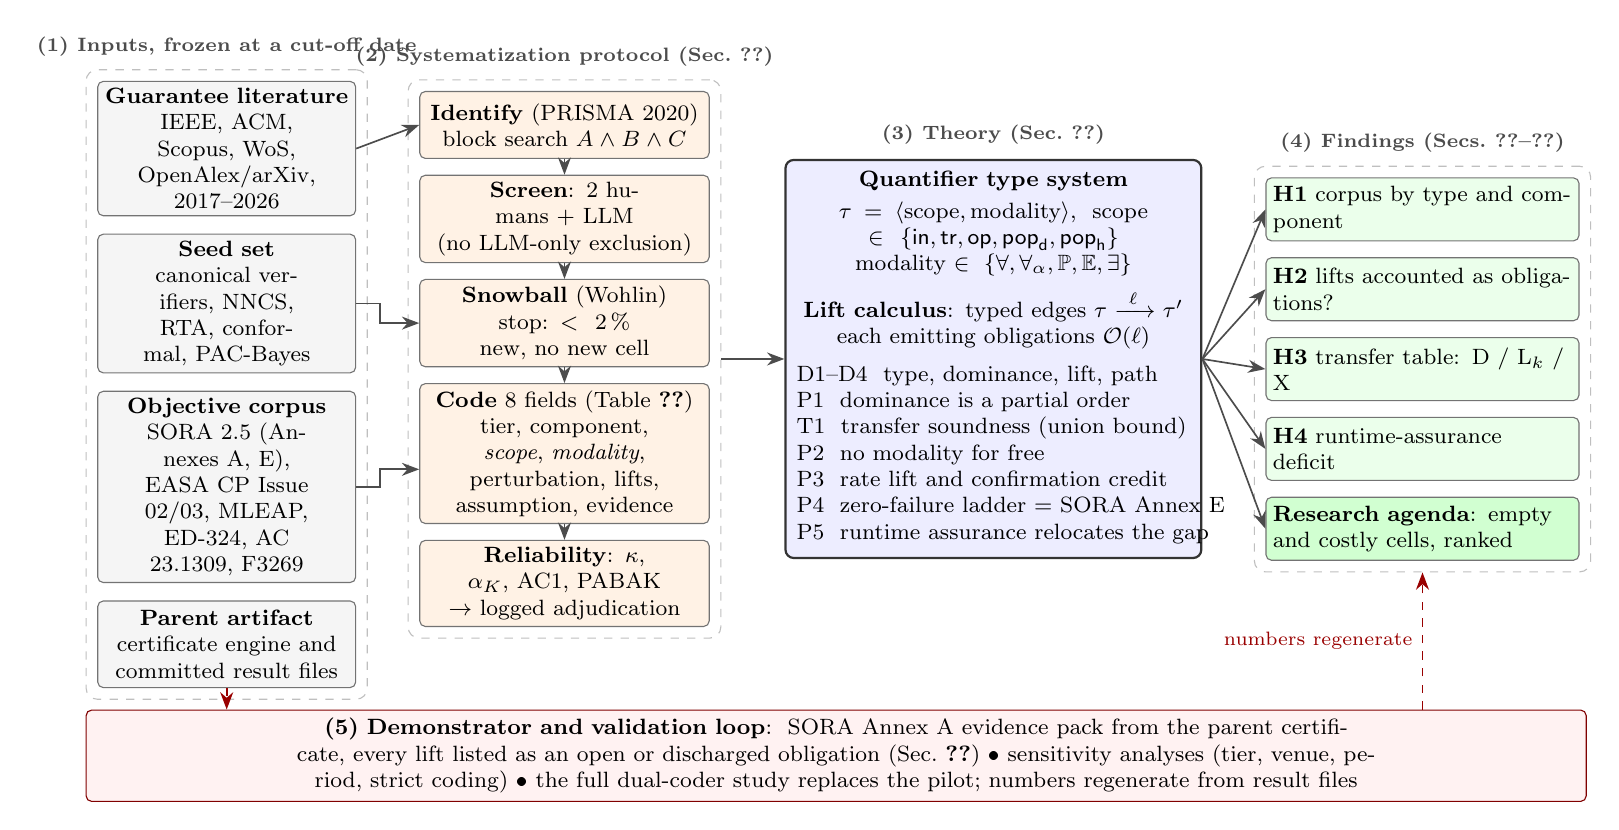
\begin{tikzpicture}[
  font=\footnotesize,
  >={Stealth[length=2.2mm]},
  inbox/.style={draw=black!55, rounded corners=2pt, fill=gray!8, align=center,
                text width=31mm, minimum height=11mm, inner sep=2.5pt},
  pstep/.style={draw=black!55, rounded corners=2pt, fill=orange!10, align=center,
               text width=35mm, minimum height=8.5mm, inner sep=2.5pt},
  core/.style={draw=black!80, thick, rounded corners=3pt, fill=blue!7,
               align=center, text width=50mm, inner sep=4pt},
  outbox/.style={draw=black!55, rounded corners=2pt, fill=green!8, align=left,
                 text width=38mm, minimum height=8mm, inner sep=2.5pt},
  lane/.style={draw=black!25, dashed, rounded corners=4pt, inner sep=4pt},
  lbl/.style={font=\scriptsize\bfseries, text=black!70},
  flow/.style={->, draw=black!70, line width=0.6pt},
  fb/.style={->, draw=red!60!black, line width=0.6pt, dashed}
]
% ---------------- (1) inputs ------------------------------------------
\node[inbox] (lit) {\textbf{Guarantee literature}\\ IEEE, ACM, Scopus, WoS,\\ OpenAlex/arXiv, 2017--2026};
\node[inbox, below=2.2mm of lit] (seed) {\textbf{Seed set}\\ canonical verifiers, NNCS,\\ RTA, conformal, PAC-Bayes};
\node[inbox, below=2.2mm of seed] (reg) {\textbf{Objective corpus}\\ SORA 2.5 (Annexes A, E),\\ EASA CP Issue 02/03, MLEAP,\\ ED-324, AC 23.1309, F3269};
\node[inbox, below=2.2mm of reg] (par) {\textbf{Parent artifact}\\ certificate engine and\\ committed result files};
\node[lane, fit=(lit)(par)] (L1) {};
\node[lbl, above=0.4mm of L1] {(1) Inputs, frozen at a cut-off date};

% ---------------- (2) protocol ------------------------------------------
\node[pstep, right=8mm of lit, yshift=3mm] (s1) {\textbf{Identify} (PRISMA 2020)\\ block search $A\wedge B\wedge C$};
\node[pstep, below=2mm of s1] (s2) {\textbf{Screen}: 2 humans + LLM\\ (no LLM-only exclusion)};
\node[pstep, below=2mm of s2] (s3) {\textbf{Snowball} (Wohlin)\\ stop: $<2\,\%$ new, no new cell};
\node[pstep, below=2mm of s3] (s4) {\textbf{Code} 8 fields (Table~\ref{tab:codebook})\\ tier, component, \emph{scope}, \emph{modality},\\ perturbation, lifts, assumption, evidence};
\node[pstep, below=2mm of s4] (s5) {\textbf{Reliability}: $\kappa$, $\alpha_K$, AC1, PABAK\\ $\rightarrow$ logged adjudication};
\node[lane, fit=(s1)(s5)] (L2) {};
\node[lbl, above=0.4mm of L2] {(2) Systematization protocol (Sec.~\ref{sec:protocol})};

% ---------------- (3) theory core ----------------------------------------
\node[core, right=8mm of L2] (core) {\textbf{Quantifier type system}\\[2pt]
  $\tau=\langle\text{scope},\text{modality}\rangle$,\ \ scope $\in\{\mathsf{in},\mathsf{tr},\mathsf{op},\mathsf{pop}_\mathsf{d},\mathsf{pop}_\mathsf{h}\}$\\
  modality $\in\{\forall,\forall_\alpha,\mathbb{P},\mathbb{E},\exists\}$\\[4pt]
  \textbf{Lift calculus}: typed edges $\tau\xrightarrow{\ \ell\ }\tau'$\\ each emitting obligations $\mathcal{O}(\ell)$\\[4pt]
  \begin{tabular}{@{}l@{}}
  D1--D4\ \ type, dominance, lift, path\\
  P1\ \ dominance is a partial order\\
  T1\ \ transfer soundness (union bound)\\
  P2\ \ no modality for free\\
  P3\ \ rate lift and confirmation credit\\
  P4\ \ zero-failure ladder $=$ SORA Annex E\\
  P5\ \ runtime assurance relocates the gap
  \end{tabular}};
\node[lbl, above=0.6mm of core] {(3) Theory (Sec.~\ref{sec:theory})};

% ---------------- (4) outputs ---------------------------------------------
\node[outbox, right=8mm of core, yshift=19mm] (o1) {\textbf{H1} corpus by type and component};
\node[outbox, below=2mm of o1] (o2) {\textbf{H2} lifts accounted as obligations?};
\node[outbox, below=2mm of o2] (o3) {\textbf{H3} transfer table: D / L$_k$ / X};
\node[outbox, below=2mm of o3] (o4) {\textbf{H4} runtime-assurance deficit};
\node[outbox, below=2mm of o4, fill=green!18] (o5) {\textbf{Research agenda}: empty and costly cells, ranked};
\node[lane, fit=(o1)(o5)] (L4) {};
\node[lbl, above=0.4mm of L4] {(4) Findings (Secs.~\ref{sec:results}--\ref{sec:agenda})};

% ---------------- flows -------------------------------------------------
\draw[flow] (lit.east) -- (s1.west);
\draw[flow] (seed.east) -- ++(3mm,0) |- (s3.west);
\draw[flow] (s1) -- (s2); \draw[flow] (s2) -- (s3); \draw[flow] (s3) -- (s4); \draw[flow] (s4) -- (s5);
\draw[flow] (reg.east) -- ++(3mm,0) |- ([yshift=-2mm]s4.west);
\draw[flow] (L2.east) -- (core.west);
\foreach \o in {o1,o2,o3,o4,o5} \draw[flow] (core.east) -- (\o.west);

% ---------------- (5) demonstrator and validation ------------------------
\path let \p1=(L1.west), \p2=(L4.east), \p3=(L2.south) in
  node[draw=red!50!black, rounded corners=2pt, fill=red!5, align=center,
       text width={\x2-\x1-8pt}, inner sep=3pt, anchor=north west] (val)
  at (\x1,\y3-9mm)
 {\textbf{(5) Demonstrator and validation loop}:\ \
  SORA Annex A evidence pack from the parent certificate, every lift listed as an open or discharged obligation (Sec.~\ref{sec:case})\ \textbullet\
  sensitivity analyses (tier, venue, period, strict coding)\ \textbullet\
  the full dual-coder study replaces the pilot; numbers regenerate from result files};
\draw[fb] (par.south) -- (par.south |- val.north);
\draw[fb] (L4.south |- val.north) -- (L4.south)
  node[midway, left, font=\scriptsize, text=red!60!black]{numbers regenerate};
\end{tikzpicture}}
\caption{Methodological framework. (1)~Two corpora enter the study: guarantees about learned
components, and assurance objectives from aviation regulation and standards, both frozen at a
cut-off date. (2)~A registered protocol identifies, screens, snowballs and codes the
guarantees. Two coders work independently, a language model acts as a logged third coder, and
reliability is reported per field before adjudication. (3)~Every guarantee and objective
receives a quantifier type, and a calculus of typed lifts computes, for each pair, whether the
guarantee discharges the objective, needs lifts whose assumptions become obligations, or is a
category error. (4)~The coded corpus and the calculus answer H1--H4 and yield a ranked research
agenda. (5)~An evidence generator instantiates one sound path end to end, and the validation
loop regenerates every number from result files.}
\label{fig:framework}
\end{figure*}


% =====================================================================
\section{Methodology I: A Quantifier Type System}
\label{sec:theory}
% =====================================================================
The framework (Fig.~\ref{fig:framework}) has five stages. This section develops stage~(3),
the theory against which the corpus is coded. Section~\ref{sec:protocol} develops
stages~(1), (2) and~(5). Proofs omitted here are in Appendix~\ref{app:proofs}.

\subsection{Types}
\begin{definition}[Quantifier type]
\label{def:type}
A guarantee or objective has type $\tau=\langle\sigma,\mu\rangle$. The \emph{scope}
$\sigma\in\{\scin,\sctr,\scop,\scpopd,\scpoph\}$ names the object quantified over: inputs in a
neighbourhood or region of one point ($\scin$), trajectories over a bounded horizon ($\sctr$),
one complete operation or every execution ($\scop$), a distribution of demands such as inputs,
environments or operations ($\scpopd$), or a rate per flight hour ($\scpoph$). The
\emph{modality} $\mu\in\{\modA,\modAc,\modP,\modE,\modX\}$ names the kind of claim: sound for
all ($\modA$), for all with confidence $1-\alpha$ over the certifier's own randomness ($\modAc$),
a probability bound over the environment or data ($\modP$), a bound on an expectation ($\modE$),
or an existential witness ($\modX$).
\end{definition}

Two distinctions in Definition~\ref{def:type} carry most of the weight. First, $\modAc$ is not
$\modP$. The confidence of randomized smoothing is over the certifier's coins. It says nothing
about how often the aircraft meets an input outside the certified ball. Second, $\scpopd$ is not
$\scpoph$. A misclassification probability per image, or a failure probability per mission, is
a statement per demand. A target per flight hour also needs an exposure model. Fig.~\ref{fig:lattice}
draws the type plane.

\subsection{Dominance}
\begin{definition}[Dominance]
\label{def:dom}
Type $\tau$ \emph{dominates} $\tau'$, written $\tau\dom\tau'$, if a statement of type $\tau$
entails a statement of type $\tau'$ about the same property with no further evidence. A
guarantee $g$ \emph{discharges} an objective $o$ if $\tau_g\dom\tau_o$ and the perturbation model
of $g$ covers the hazard of $o$.
\end{definition}

Dominance is generated by two obligation-free rules. A probability bound on a failure event is a
bound on the expectation of its indicator, so $\langle\sigma,\modP\rangle\dom\langle\sigma,\modE\rangle$
for population scopes. A probability bound per operation is a statement about the population of
operations, so $\Q{op}{P}\dom\Q{popd}{P}$.

\begin{proposition}[Dominance is a partial order]
\label{pr:order}
$\dom$ is reflexive, transitive and antisymmetric. Under it, $\Q{in}{A}$ and $\Q{poph}{P}$ are
incomparable, and so are $\Q{op}{A}$ and $\Q{popd}{P}$.
\end{proposition}

The proposition is the formal content of the gap. Under $\dom$, a radius is not a weaker or
stronger kind of per-flight-hour claim. It is a different claim, and moving between the two is
an argument, not a weakening. The second incomparability surprises at first: a per-operation
``for all'' looks stronger than any probability. It is stronger only on its certified set. To
become a probability over deployed operations, it needs evidence that deployed operations stay
in that set.

\subsection{Lifts and Obligations}
\begin{definition}[Lift]
\label{def:lift}
A \emph{lift} $\ell:\tau\to\tau'$ is an inference rule whose premise is a statement of type
$\tau$ and whose conclusion is a statement of type $\tau'$. It is valid only together with a set
of side conditions $\Obl(\ell)$, its \emph{obligations}. Each obligation has an evidence kind:
\emph{proof}, \emph{model}, \emph{statistical}, or \emph{architectural}.
\end{definition}

Table~\ref{tab:lifts} lists the seven lifts of the calculus. Each one corresponds to a family of
arguments in the corpus. \lift{dyn} is the Lipschitz--Gr\"onwall step of the running
example~\cite{gronwall1919} and the reachability step of NNCS verification. \lift{op} is the
operational-profile argument of reliability assessment~\cite{zhao2021ram,dong2023reliability}.
\lift{sup} is the argument, usually left implicit, that deployed operations stay inside the
certified set. \lift{mon} is the Simplex argument~\cite{sha2001simplex,mehmood2022bbsimplex}.

\begin{table*}[t]
\centering
\caption{The lift calculus. Each lift is an inference rule from a premise type to a conclusion
type, valid together with its obligations. Kind: \textsc{p} proof, \textsc{m} model,
\textsc{s} statistical, \textsc{a} architectural. The rules are implemented as the edge set of
\texttt{quantifier.py}, and the propositions are checked on it mechanically.}
\label{tab:lifts}
\footnotesize
\renewcommand{\arraystretch}{1.1}
\begin{tabularx}{\textwidth}{@{}l >{\raggedright\arraybackslash}p{0.2\textwidth} X >{\raggedright\arraybackslash}p{0.22\textwidth} c@{}}
\toprule
Lift & Edge & Rule (premise $\Rightarrow$ conclusion) & Obligations & Kind \\
\midrule
\lift{\alpha} & $\langle\sigma,\modAc\rangle\to\langle\sigma,\modA\rangle$ & certificate valid with probability $1-\alpha$ over the certifier's coins $\Rightarrow$ certificate valid, at confidence $1-\alpha$ & \obl{\alpha}: accept $\alpha$ & \textsc{p} \\
\lift{dyn} & $\Q{in}{A}\to\Q{tr}{A}$ & $\|\delta u(t)\|\le r$ for all $t$, drift $L$-Lipschitz $\Rightarrow$ $\|e(t)\|\le r(e^{Lt}-1)$ on $[0,T_c]$ & \obl{lip}: $L$ and model error over the operating region & \textsc{m} \\
\lift{hor} & $\Q{tr}{A}\to\Q{op}{A}$; $\Q{tr}{P}\to\Q{op}{P}$ & tube bound per window, re-anchoring every $T_c$ $\Rightarrow$ bound on $\sup_{[0,T]}\|e\|$ & \obl{hor}: re-anchoring or horizon covers the operation & \textsc{m} \\
\lift{op} & $\langle\scin,\modA|\modP\rangle\to\Q{popd}{P}$ & robust on cells $c\in\mathcal{C}$ $\Rightarrow$ $\Pr_{x\sim\mathrm{OP}}[\text{error}]\le \mathrm{OP}(\mathcal{X}\setminus\cup\mathcal{C})+\varepsilon_{\mathrm{prof}}$ & \obl{prof}: operational profile and per-cell robustness & \textsc{s} \\
\lift{sup} & $\Q{op}{A}\to\Q{popd}{P}$ & $\varphi(\omega)$ for all $\omega\in S$ $\Rightarrow$ $\Pr_{\omega\sim D}[\neg\varphi]\le\Pr_D[\omega\notin S]\le\varepsilon_{\mathrm{odd}}$ & \obl{odd}: deployment stays in the certified set & \textsc{s} \\
\lift{rate} & $\Q{popd}{P}\to\Q{poph}{P}$ & per-demand hazard $\le p$, $n_d$ demands per hour $\Rightarrow$ $\lambda\le n_dp$ (Prop.~\ref{pr:rate}) & \obl{dep}: exposure $n_d$, stationarity; dependence model for confirmation credit & \textsc{s} \\
\lift{mon} & $\langle\scin,\modA|\modP\rangle\to\Q{op}{P}$ & monitor flags hazardous inputs, switch within latency, verified recovery $\Rightarrow$ per-operation safety except on monitor misses & \obl{mcov}, \obl{lat}, \obl{rec}, \obl{ind} & \textsc{s,m,p,a} \\
\midrule
\multicolumn{5}{@{}l}{\emph{Free edges} (no obligation): $\Q{op}{P}\to\Q{popd}{P}$ (identity of reading); $\langle\scpop_\cdot,\modP\rangle\to\langle\scpop_\cdot,\modE\rangle$ (indicator expectation).} \\
\multicolumn{5}{@{}l}{\emph{Hazard coverage}: \obl{thr} is added whenever the guarantee's perturbation model does not cover the objective's hazard (natural, adversarial, or both).} \\
\bottomrule
\end{tabularx}
\end{table*}

\subsection{Transfer Paths and Soundness}
\begin{definition}[Transfer path and assurance deficit]
\label{def:path}
A \emph{transfer path} from guarantee $g$ to objective $o$ is a sequence of lifts
$\pi=\ell_1\cdots\ell_k$ with $\ell_1$ starting at $\tau_g$ and $\ell_k$ ending at a type that
dominates $\tau_o$. Its \emph{assurance deficit} is the obligation set
$\Obl(\pi)=\bigcup_i\Obl(\ell_i)$, extended by \obl{thr} when the hazard is not covered. The
\emph{verdict} is \textbf{D} (discharge) if some path has an empty deficit, \textbf{L}$_k$ if the
least deficit has $k$ obligations, and $\times$ (category error) if no path exists.
\end{definition}

\begin{theorem}[Transfer soundness]
\label{th:sound}
Let $g$ hold with confidence at least $1-\delta_0$, where $\delta_0=0$ for $\modA$ and
$\delta_0=\alpha$ for $\modAc$. Let $\pi$ be a transfer path from $g$ to $o$, and let each
obligation $\obl{}\in\Obl(\pi)$ be discharged by evidence that is valid with probability at
least $1-\delta_{\mathsf{O}}$, where $\delta_{\mathsf{O}}=0$ for proofs. Then the conclusion of
$\pi$ holds with confidence at least
\begin{equation}
\label{eq:sound}
1-\delta_\pi,\qquad \delta_\pi\;=\;\delta_0+\sum_{\mathsf{O}\in\Obl(\pi)}\delta_{\mathsf{O}},
\end{equation}
and its error term composes along the rules of Table~\ref{tab:lifts}, additively through
\lift{op} and \lift{sup} and multiplicatively by $n_d$ through \lift{rate}. If the conclusion's type
dominates $\tau_o$, the objective's statement holds at that confidence.
\end{theorem}

Theorem~\ref{th:sound} is elementary, a union bound over the events on which some premise fails.
Its use is accounting. A paper that lifts a guarantee without naming $\delta_{\mathsf{O}}$ for
each obligation has not established Eq.~\eqref{eq:sound}. It has established a conditional
statement whose conditions an assurance case must carry. This is H2 made measurable: the
coding scheme records, per guarantee, whether the assumption of each lift is unstated, stated,
stated and evidenced, or evidenced with a confidence that enters the final claim.

% =====================================================================
% Fig. 2 -- The type plane and the lift graph (quantifier.py, EDGES).
% Drawn at native column width (no rescaling), so labels stay legible.
% =====================================================================
\begin{figure}[t]
\centering
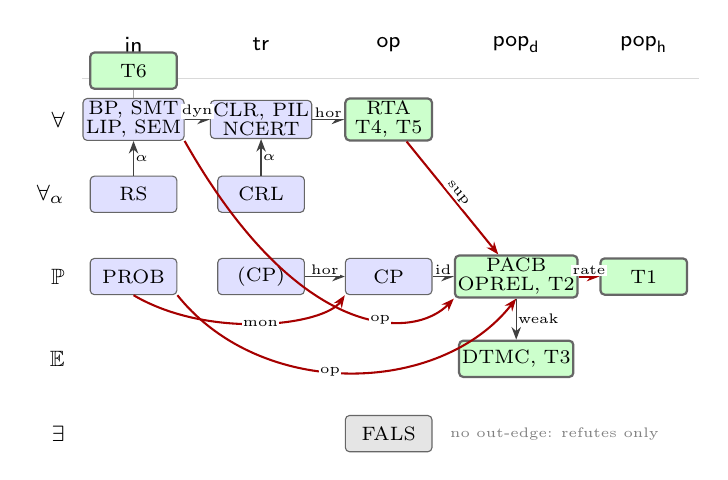
\begin{tikzpicture}[
  font=\scriptsize, >={Stealth[length=1.6mm]},
  st/.style={draw=black!60, rounded corners=1.5pt, fill=blue!12, minimum width=11mm,
             minimum height=4.6mm, inner sep=1pt, align=center},
  obj/.style={st, fill=green!20, thick},
  lf/.style={->, draw=black!75, line width=0.5pt},
  lfs/.style={->, draw=red!65!black, line width=0.75pt},
  lab/.style={font=\tiny, fill=white, inner sep=0.4pt}
]
\def\dx{1.62}
\def\dy{0.95}
% axes labels
\foreach \s/\i/\lab in {in/0/$\mathsf{in}$, tr/1/$\mathsf{tr}$, op/2/$\mathsf{op}$,
                         popd/3/$\mathsf{pop}_\mathsf{d}$, poph/4/$\mathsf{pop}_\mathsf{h}$}
  {\node[font=\footnotesize] at (\i*\dx, 4.2*\dy) {\lab};}
\foreach \m/\j/\lab in {A/3.2/$\forall$, Ac/2.2/$\forall_\alpha$, P/1.1/$\mathbb{P}$, E/0/$\mathbb{E}$, X/-1/$\exists$}
  {\node[font=\footnotesize, anchor=east] at (-0.75, \j*\dy) {\lab};}
\draw[black!15] (-0.65, 3.75*\dy) -- (4*\dx+0.7, 3.75*\dy);
% states
\node[st] (inA)   at (0*\dx, 3.2*\dy) {BP, SMT\\[-1pt]LIP, SEM};
\node[obj] (T6)   at (0*\dx, 3.2*\dy+0.62) {T6};
\node[st] (inAc)  at (0*\dx, 2.2*\dy) {RS};
\node[st] (inP)   at (0*\dx, 1.1*\dy) {PROB};
\node[st] (trA)   at (1*\dx, 3.2*\dy) {CLR, PIL\\[-1pt]NCERT};
\node[st] (trAc)  at (1*\dx, 2.2*\dy) {CRL};
\node[st] (trP)   at (1*\dx, 1.1*\dy) {(CP)};
\node[obj] (opA)  at (2*\dx, 3.2*\dy) {RTA\\[-1pt]T4, T5};
\node[st] (opP)   at (2*\dx, 1.1*\dy) {CP};
\node[st, fill=gray!20] (opX) at (2*\dx, -1*\dy) {FALS};
\node[obj] (pdP)  at (3*\dx, 1.1*\dy) {PACB\\[-1pt]OPREL, T2};
\node[obj] (pdE)  at (3*\dx, 0*\dy) {DTMC, T3};
\node[obj] (phP)  at (4*\dx, 1.1*\dy) {T1};
\draw[black!35] (T6) -- (inA);
% model / proof edges
\draw[lf] (inAc) -- node[lab, right] {$\alpha$} (inA);
\draw[lf] (trAc) -- node[lab, right] {$\alpha$} (trA);
\draw[lf] (inA)  -- node[lab, above] {dyn} (trA);
\draw[lf] (trA)  -- node[lab, above] {hor} (opA);
\draw[lf] (trP)  -- node[lab, above] {hor} (opP);
\draw[lf] (opP)  -- node[lab, above] {id} (pdP);
\draw[lf] (pdP)  -- node[lab, right] {weak} (pdE);
% statistical edges
\draw[lfs] (opA) -- node[lab, sloped, above] {sup} (pdP);
\draw[lfs] (pdP) -- node[lab, above] {rate} (phP);
\draw[lfs] (inA.south east) .. controls (1.3*\dx, 0.2*\dy) and (2.2*\dx, 0.25*\dy) .. node[lab, pos=0.62] {op} (pdP.south west);
\draw[lfs] (inP.south) .. controls (0.6*\dx, 0.25*\dy) and (1.5*\dx, 0.45*\dy) .. node[lab, pos=0.5] {mon} (opP.south west);
\draw[lfs] (inP.south east) .. controls (1.0*\dx, -0.55*\dy) and (2.4*\dx, -0.5*\dy) .. node[lab, pos=0.45] {op} (pdP.south);
\node[font=\tiny, text=gray, anchor=west, align=left] at ($(opX.east)+(0.1,0)$) {no out-edge: refutes only};
\end{tikzpicture}
\\[2pt]
{\tiny\textcolor{red!65!black}{\rule[0.5ex]{4mm}{0.8pt}} statistical obligation\quad
\textcolor{black!75}{\rule[0.5ex]{4mm}{0.5pt}} model or proof obligation\quad
\fcolorbox{black!60}{blue!12}{\strut} classes\quad
\fcolorbox{black!60}{green!20}{\strut} objective types}
\caption{The type plane. Columns are scopes, rows are modalities, and boxes place the pilot's
guarantee classes and objective types T1--T6. Each arrow is a lift with obligations
(Table~\ref{tab:lifts}). Red arrows carry a statistical obligation, and every path from a
$\forall$ state to a $\mathbb{P}$ state crosses one (Proposition~\ref{pr:nofree}). No arrow
points left, and none leaves $\exists$ or $\mathbb{E}$.}
\label{fig:lattice}
\end{figure}


\subsection{Four Structural Consequences}
\begin{proposition}[No modality for free]
\label{pr:nofree}
Every transfer path from a type with modality $\modA$ or $\modAc$ to a type with modality
$\modP$ contains at least one lift with a statistical obligation.
\end{proposition}

The proposition states something the field often argues informally~\cite{butler1993infeasibility,bensalem2023achievable},
and the calculus makes it exact. No chain of proofs, however sound or tight, turns a radius into
a probability over deployment. At some point an argument must sample the world the aircraft
will fly in. Better certificates shrink the other terms of Eq.~\eqref{eq:sound}. They cannot
remove the statistical one.

\begin{proposition}[Rate lift and confirmation credit]
\label{pr:rate}
Let a component take $f$ decisions per second, each hazardous with stationary marginal
probability at most $p$.
(a)~The expected number of hazardous decisions per flight hour is at most $3600fp$, whatever
the dependence between decisions. Hence a per-hour target $\lambda$ is met whenever
$p\le p^\star=\lambda/(3600f)$.
(b)~Suppose a hazard requires $k\ge2$ consecutive erroneous decisions. Under arbitrary
stationary dependence, the rate of hazardous runs is at most $3600fp/k$. Under a two-state
Markov error process with persistence $\rho=\Pr(e_t\mid e_{t-1})$, it equals
$3600fp(1-\rho)\rho^{k-1}\le 3600fp\,(k-1)^{k-1}/k^k$. Under independence it is approximately
$3600fp^k$.
\end{proposition}

At 30\,Hz and $10^{-4}$/FH, part~(a) gives $p^\star=\ratePstarThirty$ per frame
($\rateDecisionsPerH$ decisions per hour). At $10^{-9}$/FH it gives $p^\star=\ratePstarNine$.
Part~(b) explains a common move. Temporal filtering is credited with turning a per-frame error
of $\ratePstarKThree$ into a per-hour rate of $10^{-4}$, a gain of about $\rateGainIndep$. That
credit is real only under independence. A first-order Markov process guarantees a gain of only
$k^k/(k-1)^{k-1}=\rateGainBound$ for $k=3$, and arbitrary dependence guarantees only $k$
(Fig.~\ref{fig:rate}(b)). The obligation \obl{dep} is therefore where perception-based per-hour
arguments stand or fall.

\begin{proposition}[Zero-failure ladder]
\label{pr:ladder}
(a)~Under a homogeneous Poisson failure process, $T$ failure-free hours reject
$\lambda\ge\lambda_0$ at level $a$ if and only if $T\ge\ln(1/a)/\lambda_0$. At $a=0.05$ the SORA~2.5
Annex~E test durations of 30, 300, 3000 and 30\,000~h~\cite{jarus_sora25_E} correspond to
$\lambda_0=10^{-1},\dots,10^{-4}$/FH within $0.15\,\%$.
(b)~Demonstrating $p\le\lambda_0/(3600f)$ per frame by zero-failure testing requires exactly as
many hours of data as (a). It also replaces an independence assumption between hours with one
between frames, which is harder to defend.
\end{proposition}

Part~(a) shows that a regulator already accepts a concentration lift, the ``rule of
three''~\cite{hanley1983rule}, with explicit arithmetic. We use it as the worked example of a
regulator-endorsed $\Q{popd}{P}\to\Q{poph}{P}$ step. Part~(b) closes a tempting shortcut:
$10^{-4}$/FH at 30\,Hz needs $\ecoFramesFour$ failure-free frames, or $\ecoHoursFour$\,h, and
$10^{-7}$/FH needs about $\ecoYearsSeven$ years of continuous flight~\cite{kalra2016driving,littlewood1993validation}.

\begin{proposition}[Runtime assurance relocates the gap]
\label{pr:rta}
In the calculus, $\Q{op}{A}$ objectives are discharged directly only by a guarantee of type
$\Q{op}{A}$. Such a guarantee from runtime assurance is conditional on
$\{\obl{mcov},\obl{lat},\obl{rec},\obl{ind}\}$. When the monitor's decision depends on a learned
perception output, \obl{mcov} is a statement of type $\Q{popd}{P}$ about that output, the same
type as the gap the architecture was introduced to bridge.
\end{proposition}

\begin{corollary}[The cheapest route skips the operation]
\label{co:route}
From $\Q{in}{A}$, the least-obligation route to $\Q{poph}{P}$ is $\lift{op}\lift{rate}$, with
two obligations. It never visits $\Q{op}{A}$. Every route that also yields a per-operation
guarantee costs at least four obligations: \obl{lip}, \obl{hor}, \obl{odd} and \obl{dep}.
\end{corollary}

The corollary separates two things an applicant may want. One is a per-hour number. The other
is a per-operation envelope, which is what sizes a contingency volume. The cheaper route yields
the first without the second. The running example takes the longer route and pays for it, and
Section~\ref{sec:case} shows what it buys.

% =====================================================================
\section{Methodology II: Systematization Protocol}
\label{sec:protocol}
% =====================================================================
\subsection{The Guarantee Corpus}
\paragraph*{Sources and search}
The protocol follows the systematic-review guidelines of Kitchenham and
Charters~\cite{kitchenham2007slr} and reports with the Preferred Reporting Items for Systematic
reviews and Meta-Analyses (PRISMA) 2020~\cite{page2021prisma}. We search IEEE Xplore, the ACM
Digital Library, Scopus, Web of Science, and OpenAlex (which indexes arXiv and DBLP) for
2017--2026. Each query conjoins three blocks: A, a guarantee term (16 phrases, from ``certified
robustness'' and ``reachability analysis'' to ``conformal prediction'', ``PAC-Bayes'' and
``runtime assurance''); B, a learning term; and C, an autonomy term (Appendix~\ref{app:search}).
We add venue sweeps of IEEE S\&P, USENIX Security, CCS, NDSS, CAV, TACAS, HSCC, ICCPS, EMSOFT,
NFM, SAFECOMP, DSN, NeurIPS, ICML, ICLR, CoRL, CDC and DASC. Every request is logged with a
timestamp.

\paragraph*{Inclusion}
We include a paper if it states a formal, statistical or architectural guarantee about a learned
component, or about a system containing one, and if the object its guarantee quantifies over can
be identified. We exclude empirical attack studies without a guarantee, guarantees about
non-learned components, and theses that duplicate a journal version.

\paragraph*{Two tiers}
The inclusion rule in our proposal required evaluation on an autonomous vehicle. Applied
literally, it would exclude the canonical verifiers that define the guarantee classes, which are
evaluated on image benchmarks. We therefore code two tiers. \emph{Tier~A} contains guarantees
evaluated on a vehicle task, including standard vehicle benchmarks such as ACAS~Xu, TaxiNet,
adaptive cruise control and quadrotors. \emph{Tier~B} contains method anchors evaluated only on
generic benchmarks. Every statistic is reported for tier~A and for both tiers together, so that a
reader can see how much of a finding is carried by the anchors.

\paragraph*{Snowballing}
We snowball backward and forward from the included set, following Wohlin~\cite{wohlin2014snowballing}.
We stop when two consecutive iterations each add fewer than $2\,\%$ new inclusions \emph{and}
no iteration adds a new cell of the type plane. The second condition matters more: an SoK can
miss papers, but it should not miss a kind of guarantee.

\subsection{Codebook}
\label{sec:codebook}
The unit of coding is a guarantee, the headline claim of a paper. Table~\ref{tab:codebook} lists
the eight fields. Each uses a closed vocabulary. Three decision rules prevent the confusions
that Section~\ref{sec:theory} warns against. Randomized-smoothing confidence is coded $\modAc$,
never $\modP$. Falsification is coded $\modX$, because it can only refute. A certificate checked by
sampling over its domain is coded with \lift{conc}, because sampling has entered the claim. The
pilot added three clarifying rules, which froze the codebook at version~1.1 before the full
study (Appendix~\ref{app:codebook}).

\begin{table}[t]
\centering
\caption{Codebook (version 1.1). One row per guarantee.}
\label{tab:codebook}
\footnotesize
\begin{tabularx}{\columnwidth}{@{}lX@{}}
\toprule
Field & Values \\
\midrule
tier & A (vehicle task) / B (method anchor) \\
component & perception / estimation / control / planning / end-to-end \\
scope & $\scin$ / $\sctr$ / $\scop$ / $\scpop$ \\
modality & $\modA$ / $\modAc$ / $\modP$ / $\modE$ / $\modX$ \\
perturbation & norm / semantic / patch / disturbance / distribution / poisoning / none \\
lifts (list) & \lift{dyn}, \lift{hor}, \lift{gen}, \lift{op}, \lift{rate}, \lift{conc}, \lift{sup}, \lift{mon}, none \\
assumption & U unstated / S stated / SE stated and evidenced / SEC evidenced with a confidence that enters the claim \\
evidence & proof / measured / simulated / modelled \\
\bottomrule
\end{tabularx}
\end{table}

Two codebook lifts are not edges of the calculus. \lift{gen} (a generative, abstraction or
contract surrogate for the real sensor) and \lift{conc} (a concentration, PAC, conformal or
scenario argument from samples) change how a guarantee is \emph{obtained}, not its type. They
enter the transfer table as intrinsic obligations of the class, \obl{cov} and \obl{iid}, alongside
the obligations of the calculus edges a class's members already use.

\subsection{Coders, Reliability and the LLM Third Coder}
Two coders code every paper independently. We report, per field, percent agreement, Cohen's
$\kappa$~\cite{cohen1960kappa}, Krippendorff's nominal $\alpha$~\cite{hayes2007alpha}, Gwet's
AC1~\cite{gwet2008ac1} and PABAK, each with a percentile bootstrap interval over papers. We accept
$\alpha\ge0.80$, and $\alpha\ge0.667$ for tentative conclusions only. We report AC1 and PABAK
because the corpus is expected to be skewed toward $\scin$. Under skew, $\kappa$ and $\alpha$ can
be low despite high agreement, the prevalence paradox~\cite{byrt1993prevalence}. The set-valued
lifts field is scored per lift, as a binary variable, and by mean Jaccard similarity.
Disagreements are adjudicated by discussion, and every change is logged with its rationale.

An LLM acts as a third coder under four rules. It runs at a fixed model version with a registered
prompt and codebook. Each item is coded three times, and run-to-run agreement is reported. It
may flag a screening exclusion for human review but never exclude alone. Its agreement with the
human consensus is reported separately. Published evaluations of LLM screening report
moderate-to-substantial agreement that depends strongly on the clarity of the
criteria~\cite{dennstadt2024llmscreening,li2024llmscreening}. That dependence is why we use the
LLM as an instrument to measure, not as a coder to trust.

\subsection{The Objective Corpus}
We code $\nObj$ objectives from nine documents: the SORA~2.5 main body and Annexes~A and
E~\cite{jarus_sora25_mb,jarus_sora25_A,jarus_sora25_E}; EASA's AI concept paper Issue~02 and
Proposed Issue~03~\cite{easa_cp2,easa_cp3}; the final report of EASA's Machine Learning
Application Approval (MLEAP) project~\cite{mleap2024}; ED-324/ARP6983 at the level of
concepts~\cite{ed324}; the Federal Aviation Administration (FAA) advisory circular AC~23.1309-1E
and EASA's acceptable means of compliance AMC~25.1309~\cite{faa_ac231309,easa_amc251309}; ASTM
F3269-21~\cite{astm_f3269}; and DO-326A~\cite{do326a}. Of these, $\nObjPrimary$ were checked
against the primary text. The others, marked $\dagger$ in Table~\ref{tab:objectives}, rest on
secondary sources and are flagged for checking. Objectives with no behavioural quantifier,
such as the structural-coverage objectives of DO-178C~\cite{do178c}, are recorded but excluded
from the transfer table: they constrain the process, not the behaviour. The corpus is frozen at
7~October~2026. ED-324 and the Proposed Issue~03 were moving at that date, so we code them only
at the level of stable concepts.

\subsection{Computing the Transfer Table}
\label{sec:compute}
The objectives fall into six types, by type and hazard (Table~\ref{tab:transfer}): per flight
hour (T1), generalization over the ODD (T2), average error (T3), per operation (T4), security
threat condition (T5) and local robustness (T6). Each guarantee class receives the modal type
and modal perturbation of its adjudicated members. Its \emph{intrinsic} obligations are those of
the lifts that at least half of its members use. For each class and objective type, we compute
the least-obligation path with Dijkstra's algorithm over the edge set of Table~\ref{tab:lifts}
and add \obl{thr} when the hazard is not covered. Norm-bounded, patch, semantic and poisoning
models cover adversarial hazards; disturbance and distribution models cover natural ones. One
class-level override is documented: a Simplex guarantee holds for arbitrary behaviour of the
monitored component, but not for attacks on the monitor's own inputs, so it covers natural
hazards only.

\subsection{Pilot and Full Study}
\label{sec:pilot}
This paper reports a pilot that exercises every step of the protocol. The pilot corpus has
$\nCorpus$ guarantees ($\nTierA$ in tier~A, $\nTierB$ in tier~B) in $\nClasses$ classes. It is a
purposive seed set drawn from the canonical systems and from a scoping review, not a sample, so
its distributions illustrate the pipeline and do not estimate the field. Two LLM instances coded
it independently from the codebook, the second without access to the first's codes. One coder's
codes were then adjudicated against the other's with $\adjN$ logged changes across $\adjPapers$
papers. The full study, specified as a runbook in the artifact, replaces both LLM coders with
human coders, keeps the LLM as a third coder, and regenerates every number in
Sections~\ref{sec:results}--\ref{sec:agenda}.

\subsection{The Evidence Generator}
The generator reads a certified configuration of the running example from its committed result
files. It emits a SORA Annex~A-shaped pack in which: the ODD is the parent's measured operating
region; the position-holding term of the contingency volume is the certified tube radius under
the stated adversary; every other term of the contingency volume is an open obligation of the
operator; and every lift of Eq.~\eqref{eq:parent} appears, typed, with its obligation and status.
The last point is the generator's contribution. A compliance pack that lists the certificate but
hides its assumptions would commit exactly the category error this paper names.

% =====================================================================
\section{The Guarantee Landscape}
\label{sec:landscape}
% =====================================================================
We now systematize what each level offers, with the classes of the pilot in parentheses.
Appendix~\ref{app:classes} lists class membership.

\subsection{Per Input}
Per-input certificates are the most developed class. Complete methods decide properties over
input regions exactly~\cite{katz2017reluplex,katz2019marabou,wu2024marabou2} (SMT). Incomplete
sound methods scale through linear relaxations, branch and bound, and cutting
planes~\cite{gowal2018ibp,zhang2018crown,xu2020autolirpa,wang2021beta,zhang2022gcp,singh2019deeppoly,gehr2018ai2}
(BP). Lipschitz-constrained architectures make a certified margin a by-product of
training~\cite{tsuzuku2018lipschitz,trockman2021cayley,araujo2023sll} (LIP). Randomized smoothing
scales certification to large models, including detection and
segmentation~\cite{cohen2019certified,lecuyer2019pixeldp,salman2019provably,yang2020shapes,chiang2020detection,fischer2021segmentation}
(RS). Semantic, geometric and patch certificates replace the norm ball with a parametrized set
of rotations, illumination changes or bounded patches~\cite{balunovic2019geometric,fischer2020transformations,li2021tss,mohapatra2020semantic,lorenz2021pointcloud,xiang2021patchguard,xiang2022patchcleanser}
(SEM). These parametrized sets are the closest the literature comes to EASA's language of an
ODD. Each set is still a neighbourhood of one input, not a distribution over the operations
the aircraft will fly. The international verification-of-NN competition (VNN-COMP) standardizes
this level: its specifications are pre- and postconditions on one network~\cite{brix2024vnncomp}.

Aviation case studies sit here too. ACAS~Xu properties are checked over regions of encounter
geometry~\cite{katz2017reluplex,julian2019acasxu}. Industrial studies have assessed an exact
ACAS~Xu implementation against draft ED-324 objectives, with formal verification discharging
some learning-assurance objectives~\cite{gabreau2024acasxu,damour2021acasxu}. The region
quantifier makes these statements per region of state space, which is still per input in our
sense. Lifting them to an encounter needs a closed-loop model.

\subsection{Per Trajectory}
For learned \emph{control} with low-dimensional state inputs, closed-loop verification is mature
(CLR). Taylor-model, star-set, polynomial-zonotope and semidefinite methods compute reachable
tubes for NN controllers in feedback with known
plants~\cite{ivanov2019verisig,ivanov2021verisig2,tran2020nnv,lopez2023nnv2,huang2019reachnn,fan2020reachnnstar,huang2022polar,schilling2022nncs,kochdumper2023polyzono,sidrane2022overt,hu2020reachsdp,rober2022backward,everett2021reachlp}.
The ARCH-COMP category for AI and NN control systems (AINNCS) benchmarks them yearly~\cite{lopez2025archcomp}.
Its 2025 report notes that tools abstracting the problem differently produced disagreeing results
on two benchmarks, direct evidence that the quantified object itself can differ between tools.
Neural Lyapunov and barrier certificates give $\forall$-trajectory statements over a
domain~\cite{chang2019neurallyapunov,abate2021fossil,dawson2023certificates} (NCERT). Certified
reinforcement learning bounds actions or cumulative reward under bounded observation
perturbations~\cite{kumar2022policysmoothing,wu2022crop,everett2021carrl,wu2022copa} (CRL).

For learned \emph{perception} in the loop, every result rests on a surrogate (PIL). The
surrogate is a generative model that maps states to plausible images~\cite{katz2022taxi}, a
learned abstraction~\cite{hsieh2022abstractions}, a perception contract~\cite{astorga2023perception,sun2023ipc,li2023refining},
a camera model~\cite{santacruz2022nnlander}, or a composition of these~\cite{iccps2025imagenncs,semiprob2025vision,posecbc2026}.
The guarantee then covers the surrogate's range, not real images. A probabilistic analysis of
Boeing's taxiing system states plainly that it is best viewed as average-case rather than
worst-case~\cite{pasareanu2023closedloop} (DTMC). This is the pattern H2 predicts: a type-changing
lift (\lift{gen}) whose assumption, surrogate coverage, is of type $\Q{popd}{P}$.

\subsection{Per Operation}
Runtime assurance gives per-execution guarantees by switching from an unverified controller to
a verified fallback when a monitor fires~\cite{sha2001simplex,mehmood2022bbsimplex,sheikhi2024bbsimplexma,schierman2020rta,desai2019soter,hobbs2023rta}
(RTA). Shields enforce a safety specification on a learning agent's actions~\cite{alshiekh2018shielding}.
ASTM F3269 standardizes the architecture for aircraft and makes ``RTA system coverage'' an
explicit concern~\cite{astm_f3269}. Monitors for learned perception detect activation patterns
or inputs outside the training distribution~\cite{cheng2019monitor,henzinger2020outside,aslansefat2020safeml}
(MON). Their detection rates are population statements, usually reported without confidence.
Falsification searches mission specifications in signal temporal logic (STL) for
counterexamples~\cite{fainekos2009robustness,dreossi2017compositional,dreossi2019verifai,fremont2020taxi}
(FALS). It is the per-operation counterpart of testing: it can refute, never discharge.

\subsection{Per Population}
Statistical guarantees bound generalization by PAC-Bayes~\cite{mcallester1999pac,dziugaite2017nonvacuous,viallard2021pacbayesadv},
including for policies across novel environments~\cite{majumdar2021pacbayes} (PACB). Conformal
prediction calibrates trajectory predictors and STL runtime verification with distribution-free
coverage under exchangeability~\cite{angelopoulos2023gentle,lindemann2023safeplanning,lindemann2023stlrv,cairoli2023conformal,lindemann2024formalcp},
and under bounded distribution shift~\cite{zhao2024robustcp,gibbs2021aci} (CP). Probabilistic
robustness estimates the mass of a neighbourhood that is misclassified~\cite{weng2019proven,webb2019statistical,baluta2021quantitative}
(PROB). It is a population statement over a ball, not over deployment. Operational-profile
reliability assessment is the one line of work that lifts per-input robustness to a probability
of misclassification per demand. It then argues from that to system-level safety
targets~\cite{zhao2021ram,dong2023reliability,zhao2020safecomp,zhao2020operational},
alongside rare-event simulation of end-to-end systems~\cite{okelly2018rareevent,corso2021survey}
(OPREL). It is the literature's most explicit $\Q{in}{A}\to\Q{popd}{P}$ lift, and it states its
assumptions. Even so, it treats them as modelling choices rather than as obligations with a
confidence. The negative results on demonstrating ultra-high reliability by testing bound what
any of these can achieve~\cite{butler1993infeasibility,littlewood1993validation,kalra2016driving}.

% =====================================================================
\section{The Objective Landscape}
\label{sec:objectives}
% =====================================================================
Table~\ref{tab:objectives} codes the objective corpus. Three observations stand out.

\emph{Regulators quantify per flight hour, and they mix quantifiers inside one document.} SORA's
target levels of safety and containment criteria are $\Q{poph}{P}$. Its operational and
contingency volumes are $\Q{op}{A}$ geometry, and it states that the specific assurance and
integrity level (SAIL) is not quantitative~\cite{jarus_sora25_mb}. EASA asks for generalization
bounds over the ODD ($\Q{popd}{P}$) and robustness of the model ($\Q{in}{A}$) in one
learning-assurance process. In the same document, it notes that generalization-based error
estimates are quantities on average ($\Q{popd}{E}$)~\cite{easa_cp2}.

\emph{The ODD defines the domain of the population quantifier.} EASA distinguishes an operational
domain (OD) at system level from an ODD at constituent level, the latter a refinement of the
former~\cite{easa_cp2}. Under our types, the ODD is the support of $D$ in \lift{sup} and the
domain of $\mathrm{OP}$ in \lift{op}. Data completeness and representativeness objectives are
therefore the evidence that discharges \obl{odd} and \obl{prof}~\cite{mleap2024}.

\emph{Architectural mitigation is the regulators' own bridge.} SORA's ``no single failure''
criterion, AC~23.1309's equivalent, ASTM F3269, and EASA's monitoring of inputs outside the ODD
are all $\Q{op}{A}$ objectives that runtime assurance targets
directly~\cite{jarus_sora25_E,faa_ac231309,astm_f3269,easa_cp2}. Secondary commentary on the
Proposed Issue~03 reports an independent operational oversight system for higher automation
levels~\cite{easa_cp3}. We record that as $\Q{op}{A}$ and flag it for checking against the
primary text.

\begin{table*}[t]
\centering
\caption{The objective corpus, coded by type and hazard (N natural, Adv adversarial, B both).
$^\dagger$Wording rests on a secondary source and is flagged for checking. Generated from
\texttt{corpus/objectives.csv}.}
\label{tab:objectives}
\scriptsize
\renewcommand{\arraystretch}{1.05}
\begin{tabularx}{\textwidth}{@{}l>{\raggedright\arraybackslash}p{0.27\textwidth}Xlll@{}}
\toprule
ID & Document & Statement (paraphrased) & Type & Hazard & Target/FH \\
\midrule
\inputbody{tab_objectives_body}
\bottomrule
\end{tabularx}
\end{table*}

% =====================================================================
\section{Results}
\label{sec:results}
% =====================================================================
\subsection{Reliability of the Pilot Coding}
Table~\ref{tab:reliability} reports agreement between the two independent pilot coders. The
fields the findings rest on are reliable. For the type, scope times modality, Krippendorff's
$\alpha$ is $\relTypeAlpha$ (95\,\% bootstrap interval $[\relTypeAlphaLo,\relTypeAlphaHi]$). For
modality alone it is $\relModAlpha$. Two fields fall short, and both teach something. Perturbation
($\alpha=\relPertAlpha$) failed on one ambiguity, whether initial-state reachability without a
disturbance input is ``none'' or ``disturbance''. Rule CLR-1 of codebook version~1.1 resolves it.
The assumption field shows the prevalence paradox: $\relAssmAgree$ agreement but
$\kappa=\relAssmKappa$, because ``stated'' dominates. AC1 is $\relAssmAcOne$. Its lower interval
bound of $\relAssmAlphaLo$ marks it as the field the full study must watch. The lifts field has
mean Jaccard similarity $\relJaccard$.

\begin{table}[t]
\centering
\caption{Pilot inter-coder reliability over $\nCorpus$ guarantees: percent agreement, Cohen's
$\kappa$, Krippendorff's $\alpha$ with 95\,\% bootstrap interval, Gwet's AC1 and PABAK. Both
coders are independent LLM instances, so the table measures codebook clarity. Generated from
\texttt{results/reliability\_C1\_C2.csv}.}
\label{tab:reliability}
\footnotesize
\setlength{\tabcolsep}{3.5pt}
\begin{tabular}{@{}lrrcrr@{}}
\toprule
Field & \% & $\kappa$ & $\alpha$ [95\,\% CI] & AC1 & PABAK \\
\midrule
\inputbody{tab_reliability_body}
\bottomrule
\end{tabular}
\end{table}

\subsection{H1: Where Guarantees Sit}
% =====================================================================
% Fig. 3 -- Pilot corpus by component and scope (figdata/dist_*.dat)
% Fig. 4 -- Per-flight-hour arithmetic (figdata/rate_*.dat)
% =====================================================================
\begin{figure}[t]
\centering
\begin{tikzpicture}
\begin{groupplot}[group style={group size=2 by 1, horizontal sep=6mm, yticklabels at=edge left},
  width=0.6\columnwidth, height=46mm, ybar stacked,
  symbolic x coords={perception,estimation,control,planning,end2end},
  xtick=data, x tick label style={rotate=40, anchor=east, font=\scriptsize},
  ymin=0, ymax=46, ylabel style={font=\scriptsize}, yticklabel style={font=\scriptsize},
  title style={font=\scriptsize, yshift=-1ex}, enlarge x limits=0.15,
  legend style={font=\scriptsize, at={(1.0,1.0)}, anchor=north east, draw=none, fill=white, fill opacity=0.85, text opacity=1}]
\nextgroupplot[title={(a) Tiers A and B}, ylabel={guarantees}]
\addplot+[fill=blue!55, draw=black!60] table[x=component, y=in] {figdata/dist_AB.dat};
\addplot+[fill=orange!60, draw=black!60] table[x=component, y=tr] {figdata/dist_AB.dat};
\addplot+[fill=green!50!black!45, draw=black!60] table[x=component, y=op] {figdata/dist_AB.dat};
\addplot+[fill=gray!45, draw=black!60] table[x=component, y=popd] {figdata/dist_AB.dat};
\nextgroupplot[title={(b) Tier A only}]
\addplot+[fill=blue!55, draw=black!60] table[x=component, y=in] {figdata/dist_A.dat};
\addplot+[fill=orange!60, draw=black!60] table[x=component, y=tr] {figdata/dist_A.dat};
\addplot+[fill=green!50!black!45, draw=black!60] table[x=component, y=op] {figdata/dist_A.dat};
\addplot+[fill=gray!45, draw=black!60] table[x=component, y=popd] {figdata/dist_A.dat};
\legend{$\mathsf{in}$, $\mathsf{tr}$, $\mathsf{op}$, $\mathsf{pop}$}
\end{groupplot}
\end{tikzpicture}
\caption{The pilot corpus by component and scope after adjudication. (a)~Across both tiers,
perception guarantees are mostly per input and control guarantees mostly per trajectory.
(b)~Among guarantees evaluated on vehicles (tier A), perception is dominated by closed-loop
verification through surrogates. The pilot was seeded purposively, so these shares illustrate
the pipeline and do not estimate the field (Sec.~\ref{sec:limits}). Provenance: \prov{pilot coding}.}
\label{fig:dist}
\end{figure}

\begin{figure}[t]
\centering
\begin{tikzpicture}
\begin{groupplot}[group style={group size=2 by 1, horizontal sep=13mm},
  width=0.58\columnwidth, height=46mm, xlabel style={font=\scriptsize}, ylabel style={font=\scriptsize},
  ticklabel style={font=\scriptsize}, title style={font=\scriptsize, yshift=-1ex}, grid=major, grid style={gray!20}]
\nextgroupplot[title={(a) per-decision requirement}, xmode=log, ymode=log, xlabel={decision rate $f$ (Hz)},
  ylabel={largest $p$ per decision}, ymin=1e-21, ymax=1e-5, xmin=1, xmax=100,
  legend style={font=\tiny, at={(0.02,0.02)}, anchor=south west, draw=none, fill=white, fill opacity=0.8, text opacity=1}, legend columns=2]
\addplot[thick, blue!70!black] table[x=f, y=l0] {figdata/rate_req.dat};
\addplot[thick, orange!80!black] table[x=f, y=l1] {figdata/rate_req.dat};
\addplot[thick, green!45!black] table[x=f, y=l2] {figdata/rate_req.dat};
\addplot[thick, red!70!black] table[x=f, y=l3] {figdata/rate_req.dat};
\addplot[thick, black, dashed] table[x=f, y=l4] {figdata/rate_req.dat};
\legend{$10^{-3}$/h, $10^{-4}$/h, $10^{-5}$/h, $10^{-7}$/h, $10^{-9}$/h}
\nextgroupplot[title={(b) credit for 3-of-3 confirmation}, ymode=log, xlabel={error persistence $\rho$},
  ylabel={gain over $k{=}1$}, xmin=0, xmax=1, ymin=1, ymax=3e6, ytick={1,10,100,1e4,1e6}]
\addplot[thick, blue!70!black, mark=*, mark size=1.2pt] table[x=rho, y=gain] {figdata/rate_corr.dat};
\addplot[dashed, red!70!black, domain=0:1] {6.75};
\addplot[dashdotted, gray, domain=0:1] {3};
\addplot[dotted, black, thick, domain=0:1] {1.05e6};
\node[font=\tiny, anchor=south, text=red!70!black] at (axis cs:0.45,7.5) {Markov floor 6.75};
\node[font=\tiny, anchor=north] at (axis cs:0.45,9e5) {independence ($\approx10^{6}$)};
\node[font=\tiny, anchor=north, text=gray] at (axis cs:0.45,2.9) {any dependence: $k=3$};
\end{groupplot}
\end{tikzpicture}
\caption{The arithmetic of the per-flight-hour quantifier. (a)~Largest per-decision hazard
probability compatible with a per-hour target, $p^\star=\lambda/(3600f)$ (Proposition~\ref{pr:rate}(a)).
At 30\,Hz and $10^{-4}$/h it is $\ratePstarThirty$. (b)~What temporal confirmation buys at
30\,Hz and $10^{-4}$/h. Under independence the gain is about $10^{6}$. Under a first-order
Markov error process the gain is never below $6.75$, whatever the persistence $\rho$, and under
arbitrary stationary dependence it is only guaranteed to be $k=3$ (Proposition~\ref{pr:rate}(b)). Provenance: \prov{derived} (closed form).}
\label{fig:rate}
\end{figure}


Fig.~\ref{fig:dist} shows the adjudicated pilot by component and scope. Across both tiers,
$\hOnePercInAB$ of the $\hOneNPercAB$ perception guarantees quantify per input, against
$\hOneCtrlInAB$ of the $\hOneNCtrlAB$ control guarantees. For control, $\hOneCtrlTrAB$ quantify
per trajectory. H1 holds for perception and fails for control, as predicted, and the type plane
should be read separately for the two. One qualification matters more than the headline. Among
tier-A perception guarantees, those evaluated on vehicles, only $\hOnePercInA$ are per input,
because vehicle-facing perception work is dominated by closed-loop verification through
surrogates. The literature has therefore moved beyond the per-input level for perception, but
only through a lift whose assumption is statistical. H1 in its original form is too coarse. The
refined statement is that per-input certificates dominate perception methods, while
vehicle-facing perception results are per trajectory \emph{conditional on} a $\Q{popd}{P}$
surrogate assumption. Whether the full corpus confirms the tier-A share is the first thing it
must settle, because the pilot over-samples closed-loop work by design.

\subsection{H2: Are Lifts Accounted For?}
Of the $\hTwoNLifted$ pilot guarantees that use at least one lift, $\hTwoShareU$ leave the lift's
assumption unstated and $\hTwoShareS$ state it without evidence. $\hTwoShareSe$ evidence it, and
only $\hTwoShareSec$ carry that evidence's confidence into the final claim. In total
$\hTwoAccounted$ account for the assumption as an obligation in the sense of
Theorem~\ref{th:sound}. The rate differs by lift. The dynamics lift is the most common
($\hTwoDynN$ papers) and is evidenced in $\hTwoDynAcc$ of them: the plant model is stated and
taken as given. The surrogate lift is evidenced in $\hTwoGenAcc$ of $\hTwoGenN$ papers, the
concentration lift in $\hTwoConcAcc$ of $\hTwoConcN$, and the monitor lift in $\hTwoMonAcc$ of
$\hTwoMonN$. No pilot paper uses \lift{sup} explicitly ($\hTwoSupN$), even though every
per-operation guarantee needs it to reach a population objective. H2 is supported, and the
pattern is sharper than predicted. The lift most often left as an assumption is the one regulators
care most about: that deployment stays inside the certified set.

There is a trend. Among lifted guarantees from 2017--2021, $\hTwoAccEarly$ account for their
assumption (n\,=\,$\hTwoNEarly$). From 2022--2026 the figure is $\hTwoAccLate$
(n\,=\,$\hTwoNLate$). Conformal methods under distribution shift, semi-probabilistic
vision controllers, and learned perception contracts all make the surrogate's assumption a
calibrated, confidence-carrying term. The full study must test whether this trend survives an
unbiased sample.

\subsection{H3: The Transfer Table}
Table~\ref{tab:transfer} is the computed transfer table. Of its $\ttCells$ cells, $\ttD$ are
discharges, $\ttL$ need lifts, and $\ttX$ are category errors. Four patterns stand out.

\emph{No class discharges a per-flight-hour objective (T1).} $\ttTOneReach$ of $\nClasses$ classes
reach T1, at least through \lift{rate}, so no per-hour claim exists without exposure and
dependence evidence. The cheapest classes (CP, PACB, OPREL) need only that one lift, which
matches H3's prediction that statistical guarantees are the natural fit. Every per-input class
needs three or four obligations. Proposition~\ref{pr:nofree} is visible in the column: every
T1 path carries a statistical obligation.

\emph{Statistical guarantees for perception are scarce.} The pilot holds $\hThreeNP$ guarantees
with modality $\modP$. $\hThreePercP$ concern perception ($\hThreePercShareP$ of perception
guarantees), and only $\hThreePercPA$ of those are evaluated on vehicles. Estimation, mostly
conformal trajectory prediction, is the exception at $\hThreeEstShareP$. Only $\hThreeNRate$
pilot papers perform the rate lift to a per-hour or per-demand system figure. H3 is supported.

\emph{Local robustness objectives (T6) are never discharged.} EASA and MLEAP robustness refers to
both natural and adversarial perturbations. Every per-input class covers one of them, so every
cell carries \obl{thr}. This is a modelling gap, not a proof gap: the certified sets of the
literature were designed for an adversary that the objective does not single out.

\emph{Falsification and average-case analyses discharge nothing above their own type.} The
FALS row is all $\times$, and DTMC discharges only the average-error objective T3. This is the
formal version of a familiar warning, that a failed search for counterexamples and an average
case are not evidence for a worst-case or tail objective.

\begin{table*}[t]
\centering
\caption{The computed transfer table. Rows are guarantee classes with their pilot size $n$ and
modal type. Columns are objective types: T1 per flight hour $\Q{poph}{P}$, T2 ODD generalization
$\Q{popd}{P}$, T3 average error $\Q{popd}{E}$, T4 per operation $\Q{op}{A}$ (N), T5 security
threat condition $\Q{op}{A}$ (Adv), T6 local robustness $\Q{in}{A}$ (B). \textbf{D}: discharge.
L$_k$: least path with $k$ obligations, lifts listed (thr: hazard coverage only).
$\times$: category error. Last column: share of class members whose lift assumption is evidenced
(SE or SEC). Generated by \texttt{corpus\_analysis.py}.}
\label{tab:transfer}
\scriptsize
\setlength{\tabcolsep}{3pt}
\renewcommand{\arraystretch}{1.25}
\begin{tabular}{@{}lrc*{6}{>{\centering\arraybackslash}p{0.098\textwidth}}r@{}}
\toprule
Class & $n$ & type & T1 per FH & T2 ODD gen. & T3 average & T4 per op. & T5 security & T6 local rob. & ev.\,\% \\
\midrule
\inputbody{tab_transfer_body}
\bottomrule
\end{tabular}
\end{table*}

\subsection{H4: Runtime Assurance}
Of the $\nClasses$ classes, $\hFourReach$ reach a per-operation objective (T4), and only RTA
discharges one directly. This is H4's prediction, but Proposition~\ref{pr:rta} qualifies it. RTA
carries $\hFourRtaDeficit$ intrinsic obligations: monitor coverage, switching latency, verified
recovery and independence. No pilot RTA paper evidences all four, and the evidenced share for the
class is zero. For a perception-based monitor, coverage is a $\Q{popd}{P}$ statement about the
monitor's learned input, so the architecture has moved the original gap onto its own monitor.
H4 is supported in the form ``RTA is the only direct bridge, and it relocates the deficit''. It
is not supported in the stronger form ``RTA closes the gap''. The independence obligation is
where the two forms part. If the monitor reads the same perception channel it guards, the
failures are common-cause and the lift collapses.

\subsection{What the Per-Flight-Hour Quantifier Costs}
Fig.~\ref{fig:rate} turns Propositions~\ref{pr:rate} and~\ref{pr:ladder} into numbers. Panel~(a)
is the budget that a per-frame argument must meet. At 30\,Hz it is $\ratePstarThirty$ for
$10^{-4}$/FH, and $\ratePstarNine$ for $10^{-9}$/FH. No certified-radius result in the corpus
speaks to a quantity of this kind, because a radius bounds no probability. Panel~(b) shows why the
usual escape, temporal confirmation, needs \obl{dep}. Without independence evidence, three-frame
confirmation is guaranteed to buy between $3$ and $\rateGainBound\times$, not the $10^{6}\times$
that the independence calculation suggests.

% =====================================================================
\section{Case Study: An Evidence Pack for the Running Example}
\label{sec:case}
% =====================================================================
We apply the generator to the composition certificate at its operating point: detector setting
$\theta=0.25$\,s, $H=2$ hops, re-anchoring horizon $T_c=1$\,s and measured local Lipschitz
constant $L=1.181$. Table~\ref{tab:pack} shows the typed chain and the pack's obligations.

\begin{table}[t]
\centering
\caption{The running example as a typed transfer path, from the generated evidence pack
(\texttt{results/evidence\_pack.json}). Status: E evidenced, P partially evidenced, S stated,
A assumed, O open.}
\label{tab:pack}
\footnotesize
\setlength{\tabcolsep}{3pt}
\begin{tabularx}{\columnwidth}{@{}l l l X c@{}}
\toprule
Step & Lift & Type & Obligation and evidence & St. \\
\midrule
$\theta\mapsto\Delta$ & Lemma & $\Q{in}{A}$ & proved; cap measured over 15\,392 hops & E \\
$\Delta\mapsto\delta$ & calibration & $\Q{in}{A}$ & $\gamma$ transfers to deployment: 3 real flights, one airframe, hover & P \\
$\delta\mapsto\rho$ & \lift{dyn} & $\Q{tr}{A}$ & \obl{lip}: local $L$ measured on the checkpoint & E \\
$\rho\mapsto$ corridor & \lift{hor} & $\Q{op}{A}$ & \obl{hor}: re-anchoring every $T_c$; delay adversary only & A \\
corridor $\mapsto$ MCR & \lift{sup} & $\Q{popd}{P}$ & \obl{odd}: mission distribution named, simulated & S \\
MCR $\mapsto$ per FH & \lift{rate} & $\Q{poph}{P}$ & \obl{dep}: not claimed & O \\
\midrule
hazard & --- & --- & \obl{thr}: delay adversary below threshold; denial, insider and monitor-input attacks not covered & S \\
\bottomrule
\end{tabularx}
\end{table}

\paragraph*{What the pack certifies}
With the empirically calibrated rate $\gamma=\epGammaEkf$\,m/s, the induced perturbation is
$\epDeltaPos$\,m, and the tube radius is $\rho=\epTubeEkf$\,m. Taking the supremum rate over all
calibration samples ($\gamma=\epGammaSup$\,m/s) gives $\epTubeSup$\,m. The position-holding term
of the SORA contingency volume under the stated adversary is therefore certified at the
$5$, $10$ and $20$\,m margins, and not at $2$\,m. Under the kinematic worst case it would be
$\epTubeKin$\,m, and nothing would be certified. The pack writes the other contingency-volume
terms (navigation accuracy, map error, reaction distance, contingency manoeuvre) as operator
obligations, because the certificate says nothing about them.

\paragraph*{What it does not certify}
Of the pack's $\epNObl$ obligations, $\epNOpen$ are open or assumed. The chain is a valid
transfer path to $\Q{op}{A}$ (T4) and, through \lift{sup}, to $\Q{popd}{P}$ (T2). It stops there:
\obl{dep} is open, so the pack supports no per-flight-hour claim, and it says so. The case also
illustrates Corollary~\ref{co:route}. The parent pays four obligations where two would buy a
per-hour number, and in return it obtains the per-operation envelope that sizes a contingency
volume. Neither route is wrong. The pack makes the choice visible.

\paragraph*{Why this reframes a limitation}
The parent bounds a proportion of missions, not a single flight, and a reviewer can read that as
a weakness. In the type plane it is the correct level for an airworthiness argument. Every
$\Q{poph}{P}$ objective is a population statement, and the only per-operation statement the
parent could add is the $\Q{op}{A}$ corridor bound it already proves. This is a reframing, and
we present it as one. It does not close the parent's interface-calibration limitation, which
remains the pack's only partially evidenced obligation.

% =====================================================================
\section{Research Agenda}
\label{sec:agenda}
% =====================================================================
The empty and costly cells of Table~\ref{tab:transfer} define the agenda. We rank them by how
many objectives they would discharge.

\begin{enumerate}[leftmargin=*,itemsep=2pt,topsep=2pt]
\item \textbf{Evidence for \obl{dep}} (all T1 cells, 7 objectives). Per-hour objectives are
  reachable from every non-refuting class only through the rate lift. Temporal-dependence models
  of perception error, with confidence and validated on flight data, are the single most valuable
  missing piece. Proposition~\ref{pr:rate} shows that credit for confirmation turns on them.
\item \textbf{Reachable tubes as contingency volumes} (T4, 6 objectives). Q$_\mathsf{tr}$ tools
  could size SORA's position-holding term directly. Our search found no paper that does so; the
  evidence pack is a first instance. The missing step is \obl{hor} under realistic
  re-anchoring, including denial.
\item \textbf{Calibrated surrogate coverage} (PIL to T2, T4). Perception-in-the-loop results
  become transferable once \obl{cov} carries a confidence. Recent work does this for
  contracts and semi-probabilistic controllers; it should become the norm.
\item \textbf{Monitor coverage with confidence} (RTA and MON to T4). ASTM F3269 names coverage
  as a concern, and we found no pilot paper that evidences it with a confidence. Independence of
  the monitor's input must be argued, not assumed.
\item \textbf{Hazard models that match the objective} (all T6 cells). Robustness objectives name
  natural and adversarial perturbations together. Certified sets parametrized by the ODD, with
  an adversarial margin, would close the coverage obligation.
\end{enumerate}

% =====================================================================
\section{Related SoKs and Surveys}
\label{sec:related}
% =====================================================================
Prior systematizations catalogue one level. The SoK of Li et al.\ organizes certified robustness
for deep networks by verification and training technique, entirely at
$\scin$~\cite{li2023sok}. Liu et al.\ survey verification algorithms~\cite{liu2021algorithms}.
Brunke et al.\ and Dawson et al.\ survey safe learning-based control and learned
certificates~\cite{brunke2022safe,dawson2023certificates}. Hobbs et al.\ introduce runtime
assurance~\cite{hobbs2023rta}. Huang et al.\ and Mohseni et al.\ survey safety and trustworthiness
of deep networks~\cite{huang2020survey,mohseni2023taxonomy}. Papernot et al.\ systematize security
and privacy in ML~\cite{papernot2018sok}. Tambon et al.\ conduct a systematic review of how to
certify ML-based safety-critical systems, and are our closest methodological
precedent~\cite{tambon2022certify}. On the assurance side, Burton et al.\ name the semantic gap
between specification and learned behaviour~\cite{burton2020mindthegaps}. Ashmore et al.\
structure assurance across the ML lifecycle~\cite{ashmore2021lifecycle}. AMLAS provides
safety-case patterns~\cite{hawkins2021amlas}, and Assurance~2.0 and eliminative argumentation
make residual doubt explicit~\cite{bloomfield2020assurance2,goodenough2015eliminative}. Seshia et
al.\ set out the challenges of verified AI~\cite{seshia2022verifiedai}, and Bensalem et al.\
argue for combining statistical and formal guarantees~\cite{bensalem2023achievable}. None of
these works types claims by what they quantify over, and none treats lifts as obligations whose
deficit can be computed. That cross-level transfer analysis is our contribution. Our obligations
map onto the assumption nodes and assurance claim points of goal structuring notation
(GSN)~\cite{gsn2021,hawkins2011clear}, so a transfer path can be exported as an argument fragment.
Formally, the per-input level is a 2-safety hyperproperty~\cite{clarkson2010hyper}, and the
$\scop/\scpop$ distinction is the distinction between path quantification and probabilistic
quantification in probabilistic computation tree logic (PCTL)~\cite{hansson1994pctl}.

% =====================================================================
\section{Limitations and Threats to Validity}
\label{sec:limits}
% =====================================================================
\emph{The corpus figures are a pilot.} The pilot was seeded purposively and over-samples
closed-loop and statistical work, so its distributions do not estimate the field. Its role is to
exercise the protocol and to fix the codebook before the full study, which replaces every number
reported here.

\emph{Both pilot coders were LLMs.} Their agreement measures how unambiguous the codebook is,
not how experts read the papers. The two coders also share a training distribution, which may
inflate agreement. The full study uses two human coders and keeps the LLM as a measured third.

\emph{The calculus is ours.} The verdicts depend on the edge set. We chose edges that correspond
to arguments in the corpus, and we release the code so that a reader can add, remove or
re-weight an edge and regenerate the table. Unit weights treat all obligations alike. A
deficit weighted by evidence kind is a natural refinement.

\emph{Class-level types hide within-class spread.} A class takes its modal type. Members of
other types are visible in Appendix~\ref{app:classes} and in the released codes.

\emph{Regulatory drift.} ED-324 and the EASA Proposed Issue~03 were moving at our cut-off, and
$\nObj-\nObjPrimary$ objectives rest on secondary sources. We code concepts, not clause numbers,
and flag every secondary objective.

\emph{Construct validity.} ``Accounted for'' (SE or SEC) is a strict reading of H2. Under a
looser reading that counts any stated assumption, the share rises to the sum of the S, SE and SEC
shares. We report both, and the sensitivity analysis of the full study re-codes under each.

% =====================================================================
\section{Conclusion}
\label{sec:conclusion}
% =====================================================================
Certified robustness and airworthiness assurance do not fail to meet because one is too weak.
They quantify over different things. Once guarantees and objectives carry types, the gap becomes
computable. Lifts bridge it, and each lift leaves an obligation behind. No chain of proofs
reaches a probability objective without a statistical obligation. The cheapest route to a
per-hour number skips the per-operation envelope that sizes a contingency volume. Runtime
assurance moves the gap onto its monitor. In the pilot, the literature states most of its lift
assumptions but evidences few of them, least of all the one regulators care about: that the
aircraft stays where the certificate holds. The evidence generator shows the alternative. It
lists every assumption as an obligation, and it keeps the boundary of the claim in the pack.

% =====================================================================
\section*{Ethics Considerations}
% =====================================================================
This work involves no human subjects and no personal data. It analyses published papers and
public regulatory documents. Mapping guarantees to regulatory objectives could be misread as
certification advice. We state throughout that it is not, and the evidence generator writes
that disclaimer into every pack it emits. The LLM coding was run on bibliographic metadata and
the coders' own knowledge of published papers; no unpublished material was processed.

\section*{Open Science}
The codebook, the coded pilot corpus with both coders' codes and the adjudication log, the
objective corpus, the calculus, the analysis scripts, the evidence generator and the runbook for
the full study are released in the anonymised artifact. Every number in this paper is a macro
generated from those files.

\bibliographystyle{IEEEtran}
\bibliography{refs}

\appendices
% =====================================================================
\section{Proofs}
\label{app:proofs}
% =====================================================================
\begin{proof}[Proof of Proposition~\ref{pr:order}]
$\dom$ is the reflexive--transitive closure of the free edges, so it is reflexive and transitive.
Each free edge either increases the scope index or moves the modality from $\modP$ to $\modE$,
and no edge reverses either, so the closure has no cycles and is antisymmetric. Every edge into
$\Q{poph}{P}$ is \lift{rate}, which is not free, so no free path reaches it from $\Q{in}{A}$. No
edge decreases scope, so no path at all leads back. The same argument applies to $\Q{op}{A}$ and
$\Q{popd}{P}$, through \lift{sup}.
\end{proof}

\begin{proof}[Proof of Theorem~\ref{th:sound}]
Each lift is a valid rule: if its premise and its obligations hold, its conclusion holds. Let $F_0$
be the event that $g$ fails and $F_{\mathsf{O}}$ the event that the evidence for $\obl{}$ is
invalid. Off $F_0\cup\bigcup_{\mathsf{O}}F_{\mathsf{O}}$, induction along $\pi$ shows that every
intermediate conclusion holds. By the union bound, that event has probability at most
$\delta_\pi$. The error terms compose by substituting each rule's bound into the next. If the
final type dominates $\tau_o$, the objective follows by Definition~\ref{def:dom}.
\end{proof}

\begin{proof}[Proof of Proposition~\ref{pr:nofree}]
The edges that change the modality from $\modA$ or $\modAc$ to $\modP$ are \lift{op}, \lift{sup}
and \lift{mon}. They carry \obl{prof}, \obl{odd} and \obl{mcov}, all statistical. \lift{\alpha}
maps $\modAc$ to $\modA$, and every other edge preserves $\modP$ or leaves it. Any path that ends at
modality $\modP$ from $\modA$ or $\modAc$ must therefore cross one of the three. The released
code checks the claim exhaustively over all pairs of types.
\end{proof}

\begin{proof}[Proof of Proposition~\ref{pr:rate}]
(a)~Let $X_t$ indicate a hazardous decision. By linearity of expectation,
$\mathbb{E}\sum_{t\le 3600f}X_t=3600f\,p$ for any joint law with marginals $p$.
(b)~Every hazardous run contains at least $k$ errors, so the number of runs is at most the number
of errors divided by $k$. Taking expectations gives the first bound. For the Markov chain,
stationarity gives $\Pr(X_{t-1}=0,X_t=1)=\Pr(X_t=1,X_{t+1}=0)=p(1-\rho)$, and a run of length at
least $k$ starts at $t$ with probability $p(1-\rho)\rho^{k-1}$. The function $(1-\rho)\rho^{k-1}$
is maximized at $\rho=(k-1)/k$, with value $(k-1)^{k-1}/k^k$. Under independence
($\rho=p$) the rate is $3600fp^k(1-p)$.
\end{proof}

\begin{proof}[Proof of Proposition~\ref{pr:ladder}]
(a)~Under a Poisson process with rate $\lambda$, $\Pr(\text{no failure in }T)=e^{-\lambda T}$. The test
rejects $\lambda\ge\lambda_0$ at level $a$ if and only if $e^{-\lambda_0T}\le a$. With $a=0.05$,
$T\lambda_0=\ln20=2.996$, so $T=30,\dots,30\,000$\,h give $\lambda_0=0.0999,\dots,9.99\times10^{-5}$.
(b)~With $n$ independent Bernoulli frames, zero failures reject $p\ge p_0$ at level $a$ when
$(1-p_0)^n\le a$, that is, $n\ge\ln(1/a)/p_0$ to first order. With $p_0=\lambda_0/(3600f)$ this
is $n/(3600f)=\ln(1/a)/\lambda_0$ hours.
\end{proof}

\begin{proof}[Proof of Proposition~\ref{pr:rta}]
In the edge set, the only edges into $\Q{op}{A}$ are \lift{hor} from $\Q{tr}{A}$ and the identity,
so a direct discharge needs a guarantee already of that type. The Simplex theorem states safety
on every execution in which the monitor flags each state outside the recoverable set within the
switching latency, and the recovery controller is verified from every state it can be handed.
These are \obl{mcov}, \obl{lat} and \obl{rec}, and the monitor's input must not share the failure
modes of the channel it guards, which is \obl{ind}. When the monitor's input is a learned perception
output, the event ``the monitor flags every hazardous state'' has a probability over deployed
inputs, which is of type $\Q{popd}{P}$.
\end{proof}

\begin{proof}[Proof of Corollary~\ref{co:route}]
$\Q{in}{A}\xrightarrow{\lift{op}}\Q{popd}{P}\xrightarrow{\lift{rate}}\Q{poph}{P}$ carries
$\{\obl{prof},\obl{dep}\}$, and no path with fewer obligations exists, because every edge into
$\Q{poph}{P}$ is \lift{rate} and no free edge leaves $\Q{in}{A}$. Any path through $\Q{op}{A}$ must
enter it by \lift{hor} from $\Q{tr}{A}$, which is reached from $\Q{in}{A}$ only by \lift{dyn}, and
must leave it by \lift{sup} and then \lift{rate}. That gives $\{\obl{lip},\obl{hor},\obl{odd},\obl{dep}\}$.
The released code reproduces both paths.
\end{proof}

% =====================================================================
\section{Search Strings}
\label{app:search}
% =====================================================================
Block A (one query per phrase): ``certified robustness'', ``certifiably robust'', ``formal
verification'', ``reachability analysis'', ``runtime assurance'', ``simplex architecture'',
``conformal prediction'', ``PAC-Bayes'', ``statistical model checking'', ``scenario approach'',
``safety verification'', ``provable guarantee'', ``perception contract'', ``safety
certificate'', ``barrier certificate'', ``operational profile''.
Block B: (``neural network'' OR ``deep learning'' OR ``learning-enabled'' OR ``machine learning''
OR ``reinforcement learning'').
Block C: (``aircraft'' OR ``UAV'' OR ``UAS'' OR ``drone'' OR ``quadrotor'' OR ``autonomous
vehicle'' OR ``autonomous driving'' OR ``avionics'' OR ``airworthiness'' OR ``collision avoidance''
OR ``safety-critical'').
Years 2017--2026. Database-specific syntax is generated by \texttt{search\_corpus.py}, which
logs every request.

% =====================================================================
\section{Codebook Decision Rules}
\label{app:codebook}
% =====================================================================
\begin{enumerate}[leftmargin=*,itemsep=1pt,topsep=2pt]
\item Randomized-smoothing confidence is $\modAc$, never $\modP$.
\item Falsification and counterexample search are $\modX$. A zero-failure sampling campaign whose
  confidence enters the claim is $\modP$.
\item If a certificate over a domain is checked by sampling and the sampling enters the claim,
  add \lift{conc}.
\item A competition report inherits the scope of its benchmark category.
\item Runtime-assurance architectures with a conditional safety theorem are $\Q{op}{A}$ with
  \lift{mon}.
\item Between two candidate scopes, choose the smaller and flag it.
\item (v1.1, CLR-1) Initial-set reachability with no disturbance input has perturbation ``none''.
\item (v1.1, PIL-1) A result over a generator's latent space is ``semantic''. A result over an
  estimated perception-error set is ``distribution''.
\item (v1.1, COMP-1) A learned trajectory or intent predictor is ``estimation''.
\end{enumerate}

% =====================================================================
\section{Guarantee Classes of the Pilot}
\label{app:classes}
% =====================================================================
\begin{table}[h]
\centering
\footnotesize
\begin{tabularx}{\columnwidth}{@{}lX@{}}
\toprule
Class & Members \\
\midrule
RS & \cite{cohen2019certified,lecuyer2019pixeldp,salman2019provably,yang2020shapes,chiang2020detection,fischer2021segmentation} \\
BP & \cite{gowal2018ibp,zhang2018crown,xu2020autolirpa,wang2021beta,zhang2022gcp,singh2019deeppoly,gehr2018ai2} \\
SMT & \cite{katz2017reluplex,katz2019marabou,wu2024marabou2,julian2019acasxu,gabreau2024acasxu} \\
LIP & \cite{tsuzuku2018lipschitz,trockman2021cayley,araujo2023sll} \\
SEM & \cite{xiang2021patchguard,xiang2022patchcleanser,balunovic2019geometric,fischer2020transformations,li2021tss,mohapatra2020semantic,lorenz2021pointcloud,posecbc2026} \\
PIL & \cite{santacruz2022nnlander,katz2022taxi,hsieh2022abstractions,astorga2023perception,sun2023ipc,li2023refining,iccps2025imagenncs,semiprob2025vision} \\
DTMC & \cite{pasareanu2023closedloop} \\
CLR & \cite{ivanov2019verisig,ivanov2021verisig2,tran2020nnv,lopez2023nnv2,huang2019reachnn,fan2020reachnnstar,huang2022polar,schilling2022nncs,kochdumper2023polyzono,sidrane2022overt,hu2020reachsdp,rober2022backward,everett2021reachlp,lopez2025archcomp} \\
CRL & \cite{kumar2022policysmoothing,wu2022crop,everett2021carrl,wu2022copa} \\
NCERT & \cite{chang2019neurallyapunov,abate2021fossil} \\
CP & \cite{lindemann2023safeplanning,lindemann2023stlrv,zhao2024robustcp,cairoli2023conformal,lindemann2024formalcp} \\
RTA & \cite{mehmood2022bbsimplex,sheikhi2024bbsimplexma,schierman2020rta,desai2019soter,alshiekh2018shielding,damour2021acasxu} \\
MON & \cite{cheng2019monitor,henzinger2020outside,aslansefat2020safeml} \\
FALS & \cite{fremont2020taxi,dreossi2019verifai,dreossi2017compositional} \\
PACB & \cite{dziugaite2017nonvacuous,viallard2021pacbayesadv,majumdar2021pacbayes} \\
PROB & \cite{weng2019proven,webb2019statistical,baluta2021quantitative} \\
OPREL & \cite{okelly2018rareevent,zhao2021ram,dong2023reliability,zhao2020safecomp,zhao2020operational} \\
\bottomrule
\end{tabularx}
\end{table}

% =====================================================================
\section{Acronyms}
% =====================================================================
\begin{table}[h]
\centering
\footnotesize
\begin{tabularx}{\columnwidth}{@{}lX@{}}
\toprule
AC1 & Gwet's first-order agreement coefficient \\
ACAS Xu & airborne collision avoidance system for unmanned aircraft \\
AINNCS & AI and neural-network control systems (ARCH-COMP category) \\
AMC & acceptable means of compliance \\
BP & bound propagation \\
CP & conformal prediction \\
DTMC & discrete-time Markov chain \\
EASA & European Union Aviation Safety Agency \\
EKF & extended Kalman filter \\
EUROCAE & European Organisation for Civil Aviation Equipment \\
FAA & Federal Aviation Administration \\
FH & flight hour \\
GSN & goal structuring notation \\
IBP & interval bound propagation \\
JARUS & Joint Authorities for Rulemaking of Unmanned Systems \\
LLM & large language model \\
MCR & mission-completion rate \\
ML / NN & machine learning / neural network \\
MLEAP & Machine Learning Application Approval (EASA project) \\
NNCS & neural-network control system \\
OD / ODD & operational domain / operational design domain \\
PABAK & prevalence-adjusted bias-adjusted kappa \\
PAC & probably approximately correct \\
PCTL & probabilistic computation tree logic \\
PRISMA & Preferred Reporting Items for Systematic reviews and Meta-Analyses \\
RS & randomized smoothing \\
RTA & run-time assurance \\
SAIL & specific assurance and integrity level \\
SMT & satisfiability modulo theories \\
SoK & systematization of knowledge \\
SORA & Specific Operations Risk Assessment \\
STL & signal temporal logic \\
TLS & target level of safety \\
UAS / UAV & unmanned aircraft system / unmanned aerial vehicle \\
VNN-COMP & International Verification of Neural Networks Competition \\
\bottomrule
\end{tabularx}
\end{table}

\end{document}
